%--------------------------------------------------------------------------------------%--------------------------------------------------------------------------------------
%
%  Global settings, dont change it! (excapt additional \usepackage commands)
%  Always use PDFLatex!
%
%--------------------------------------------------------------------------------------%--------------------------------------------------------------------------------------
\documentclass[a4paper, 12pt, oneside, BCOR1cm,toc=chapterentrywithdots]{scrbook}

\usepackage{graphicx}           % use for pdfLatex
\usepackage{makeidx} % f\"{u}r Benutzung des Befehls \printindex
\usepackage[colorlinks=false]{hyperref}
\usepackage{tocbibind}
\usepackage{blindtext}
\usepackage{subfigure} 
\usepackage{acronym}
\usepackage{amsmath}
\usepackage{gensymb}
\usepackage{listings}
\hypersetup{%
bookmarksnumbered=true, hyperindex=true,
%
%Im Acrobat Reader Subtitel 1. Ebene anzeigen
bookmarksopen=true, bookmarksopenlevel=1,
%
pdfborder=0 0 0 % Keine Box um die Links!
}

% --------------------------------------------------------------
% Force Tables and List to be added in Table of Content
% --------------------------------------------------------------

\renewcommand*{\tableofcontents}{%
  	\begingroup
  	\tocsection
  	\tocfile{\contentsname}{toc}
  	\endgroup
}
\renewcommand*{\listoffigures}{%
  	\begingroup
  	\tocsection
  	\tocfile{\listfigurename}{lof}
  	\endgroup
}
\renewcommand{\listoftables}{
	\begingroup
	\tocsection
	\tocfile{\listtablename}{lot}
	\endgroup
}
\begin{document}

%--------------------------------------------------------------------------------------%--------------------------------------------------------------------------------------
%
%  Here starts the userspace !
%
%--------------------------------------------------------------------------------------%--------------------------------------------------------------------------------------

%--------titlepage
\begin{titlepage}

{
    \begin{center}
        \raisebox{-1ex}{
\includegraphics[scale=1.5]{TU_Chemnitz_positiv_gruen.pdf}}\\
    \end{center}
    \vspace{0.5cm}
}

\begin{center}

\LARGE{\textbf{Free space detection and depth estimation using fish eye camera}}\\
\vspace{1cm}


\Large{\textbf{Research Project}}\\ 
\vspace{1cm}
\vspace{0.5cm}
Faculty of Electrical Engineering and Information Technology\\
Professorship of Digital Signal Processing and Circuit Technology
\end{center}
\vspace{2cm}
Submitted by: Adarsh Mallandur\\
Student ID: 457084\\
Date: 25.03.2019\\
Supervising tutor: Dr.-Ing. Christian Wiede \\

\end{titlepage}

%---------------------------------------------------------
% Abstract
%---------------------------------------------------------

\addchap*{Abstract}
Identifying free space or safely drivable region is a fundamental task in autonomous driving. There are numerous methods to address this problem using both  computer vision and machine learning techniques. One of the most successful methods is semantic segmentation using supervised learning. But, most of these methods are based on narrow-angle pin-hole cameras. Autonomous vehicles need a wider field of view to understand the scene better, especially in urban surroundings.  However, the main drawback of this algorithm is the expensive step of collecting manually annotated pixel level labels. There are no open-source pixel-annotated fish-eye images of urban traffic scene available on the internet. This project aims at solving this problem by creating virtual urban traffic simulation using Unity and collecting both images and ground truth of the scene by moving around in the virtual car. These images are then trained on the segmentation network E-Net through the method of transfer learning to produce pixel level class predictions for fish-eye images. The project also generates RGBD depth images to train a machine learning model. The results capture the distortions in the fish-eye images very well and can be used as a possible solution for the real-time free space detection using a fish-eye camera in autonomous driving.
\\\\
\textbf{Keywords: Fish-eye camera, semantic segmentation, transfer learning, free space detection, deep learning, urban traffic simulation}

%---------------------------------------------------------
% Table of Contents, List of figures, List of Tables
%---------------------------------------------------------

\tableofcontents
\listoffigures
\listoftables

\twocolumn
\addchap{List of Abbreviations}
\begin{acronym}[Bash]
 \acro{AI}{Artificial Intelligence}
 \acro{ANNs}{Artificial Neural Networks}
 \acro{DNNs}{Deep Neural Networks}
 \acro{CNNs}{Convolutional Neural Networks}
 \acro{GPUs}{graphics processing units}
 \acro{RGBD}{Red Blue Green Depth}
 \acro{FCN}{Fully Convolutional Networks}
 \acro{ML}{Machine Learning}
 \acro{SGD}{Stochastic Gradient Descent}
 \acro{API}{Application Programming Interface}
 \acro{FOV}{Field of view}


\end{acronym}


\onecolumn
%---------------------------------------------------------
% Here starts the real work
%---------------------------------------------------------

\chapter{Introduction}
In the past few years, there has been a tremendous amount of growth in research of Artificial Intelligence (AI) related fields such as computer vision, machine learning and autonomous vehicles. Despite these advances, fully autonomous car navigation in complex environments is decades away. The reasons for this can be thought of as non-availability of AI which generalises to new problems and because most computer vision algorithms produce errors at a rate which is not acceptable for fully autonomous navigation \cite{janai2017computer}. One solution to make the algorithms less prone to errors is by enabling autonomous vehicles to perceive their environment better. In urban environments, traffic situations can be very complex and unpredictable. To make autonomous vehicles perceive their environment better, we need to have wide-angle views. This project focusses on the task of free space detection using fisheye cameras, thus providing the autonomous vehicles with a wide-angle view. 

Fisheye camera is widely used in autonomous vehicles such as for parking \cite{wang2014automatic}, vehicle surround monitoring \cite{liu2008bird}, scene-understanding \cite{haltakov2012scene}, etc. Fisheye images have strong distortions because of projecting hemisphere onto the image plane. The conventional image processing and deep learning algorithms do not take into account of these distortions and hence cannot be directly used with fisheye images. There is a lack of labelled fisheye dataset available for development of algorithms to process fisheye images. This project tries to find a solution to this problem by creating simulated fisheye images and labels. 

This project presents a Convolutional Neural Network (CNN)-based semantic segmentation solution to detect free spaces in a complex urban traffic scene using a fisheye camera. To address the problem of lack of labelled fisheye dataset, the project aims at providing a solution using the Unity software framework \cite{unity3d}. We demonstrate that a CNN-based semantic segmentation network can be trained on simulated fisheye images and then be used for inference on real-world fisheye images. 


\section{Problem statement}
 
This project aims to solve the following problems

\begin{enumerate}
	\item State-of-the-art semantic segmentation algorithms do not work on fisheye images.
	\item Lack of labelled fisheye image dataset of urban traffic scenes.
	\item It is very expensive both in terms of time as well as money to generate labels manually\cite{bearman2016s}.
\end{enumerate}

The first problem of semantic segmentation algorithms is solved by using transfer learning, where the existing pre-trained algorithm is further trained using data of the target task. The second problem of lack of fisheye image dataset is solved by creating a simulation of urban traffic scenes using Unity\cite{unity3d}. The third problem of generating labels is solved automatically since the simulations inherently create labels to each object in the virtual environment. 

\section{Structure of the project}
The main focus of this project work can be summarised as

\begin{enumerate}
	\item To study the literature of free space detection using fisheye cameras and propose a better solution.
	\item To generate labelled fisheye dataset using the Unity framework \cite{unity3d}. The dataset has both semantic layers as well as depth labels. 
	\item To use a pre-trained CNN to evaluate the fisheye dataset and then retrain the CNN to make better predictions.
\end{enumerate}




\chapter{Related work}

There are numerous research works on the problem of free space detection. The important ones are summarised in table \ref{tab:table1} and table \ref{tab:table2} according to chronological order. In the early methods such as \cite{badino2009stixel}, superpixels called stixels were extracted from stereo images which represented mainly vertical shapes as non-free space. Early usage of CNNs for this task was in \cite{alvarez2012road} where the authors used sliding window approach to train a CNN using RGB monocular images. Fisheye cameras were used for obstacle detection in \cite{hane2015obstacle}, where the method uses wheel odometry to generate weak labels before training. Hence this can be considered as weakly supervised training.

Due to the unavailability of a labelled dataset, most of the algorithms used a semi-supervised approach\cite{brust2015convolutional} \cite{sanberg2017free}\cite{hanisch2017free}\cite{tsutsui2018minimizing}. However, this method of generating weak labels is often expensive and is often noisy. 

In \cite{deng2018restricted} and \cite{saez2018cnn} the authors have converted real world fisheye dataset into synthetic dataset by applying a fisheye transformation to each image. They have used labelled datasets such as cityscapes \cite{Cordts2016Cityscapes} to generate the synthetic fisheye dataset. These methods are not so efficient since synthetic images do not have the extra field of view as compared to real fisheye images. 

Our method generates simulated fisheye images by stitching four images from four cameras and hence providing robust images and labels, which can be used to train neural networks. In this project, we demonstrate this by training the dataset on E-Net\cite{Paszke2017ENetAD}, a segmentation CNN trained on cityscapes dataset\cite{Cordts2016Cityscapes}. 
% % Example of, how to use a Table

\blindtext[1]

\begin{center}
\begin{tabular}{|c|c|c|c|}
\hline
Research study & Objective & Features & Classifier\\
\hline
Driver Gaze Zone Estimation using Convolutional Neural Networks:
A General Framework and Ablative Analysis & 80& 0.3153 & 0.4900\\
500 & 120& 0.1229& 0.1787\\
1000 & 120& 0.0680& 0.0880\\
2000 & 120& 0.0361& 0.0441\\
5000 & 140& 0.0256& 0.0305\\
5000 & 164& 0.0343& 0.0880\\
\hline
\end{tabular}
\captionof{table}{This is the caption of the table}
\label{tab:table1}
\end{center}

\blindtext[3] % Load Data from File example_tables
\begin{center}

\captionof{table}{Related research work on free space detection using fisheye camera}
\label{tab:table1}
\begin{tabular}{| p{5cm} | l |  p{4cm} | p{2cm} | p{2cm} |}
\hline
\textbf{Literature} & \textbf{Year} & \textbf{Algorithm} & \textbf{Input} & \textbf{Output}\\
\hline
The Stixel World - A Compact Medium Level Representation of the 3D-World \cite{badino2009stixel} & 2009 & Dense stereo algorithm and stixel extraction & RGB Stereo images & Stixels\\
\hline
Road scene segmentation from a single image \cite{alvarez2012road} & 2012 & CNN trained using noisy labels. Sliding window approach is used & RGB monocular camera images & Patch labels\\ 
\hline
Obstacle detection for self-driving cars using only monocular cameras and wheel odometry \cite{hane2015obstacle} & 2015 & Depth map computation using plane sweeping and obstacle extraction & RGB Fisheye images and wheel odometry  & Occupancy grids\\
\hline
\end{tabular}
\end{center}

\begin{center}
\captionof{table}{Related research work on free space detection using fisheye camera (continued.)}
\label{tab:table2}
\begin{tabular}{| p{5cm} | l |  p{4cm} | p{2cm} | p{2cm} |}
\hline
\textbf{Literature} & \textbf{Year} & \textbf{Algorithm} & \textbf{Input} & \textbf{Output}\\
\hline
Convolutional patch networks with spatial prior for road detection and urban scene understanding \cite{brust2015convolutional}  & 2015 & Convolutional patch network using normalized position of patch as additional input & RGB Monocular camera images & Pixel labels\\
\hline
Free-space detection with self-supervised and online trained fully convolutional networks \cite{sanberg2017free}  & 2017 & FCN and self-supervised learning using weak labels from Stixel algorithm & RGB Stereo camera images & Pixel labels (Segmentation mask)\\
\hline
Free-space detection with fish-eye cameras \cite{hanisch2017free}  & 2017 & Segmentation and Random forest classification of superpixels & RGB monocular fisheye camera images & Labelled superpixels\\
\hline
CNN based semantic segmentation for urban traffic scenes using fisheye camera \cite{deng2017cnn}  & 2017 & Semantic segmentation using OPP-Net & RGB monocular fisheye images & Pixel labels (Segmentation mask)\\
\hline
Minimizing Supervision for Free-space Segmentation \cite{tsutsui2018minimizing}  & 2018 & FCN (SegNet) and weakly supervised annotation extraction & RGB monocular camera image & Pixel labels (Segmentation mask)\\
\hline
Cnn-based fisheye image real-time semantic segmentation \cite{saez2018cnn}  & 2018 & Efficient Residual Factorized CNN (ERFNet) modified with fish eye camera images & RGB monocular fisheye camera images & Pixel labels (Segmentation mask)\\
\hline
Restricted deformable convolution based road scene semantic segmentation using surround view cameras \cite{deng2018restricted}  & 2018 & Restricted Deformable Convolution (RDC) and zoom augmentation to generate fisheye images & RGB monocular fish eye camera images & Pixel labels (Segmentation mask)\\
\hline
\end{tabular}

\end{center}

\chapter{Background}
 In this chapter, we discuss the theoretical concepts of neural networks, computer vision and deep learning required for understanding the implementation of the project. First, the details of artificial intelligence, machine learning and deep learning are discussed. Finally, the application of deep learning to computer vision is examined in detail. 
 
 \section{Machine learning}
 
Machine learning is used to solve a wide variety of problems in computer vision, speech processing, statistics etc,. It is a subset of artificial intelligence where the computer is shown data to learn patterns and solve the given problem without being explicitly programmed to do so \cite{awad2015efficient}. Computers have been successful in several tasks that were considered impossible by humans. However, they fail to do simple tasks such as recognising objects or speech. Hence, machine learning algorithms were designed to infer the result from features of the input. In most of the cases, these features needed to be hand-crafted by an expert. The algorithms work better when given better features. As the availability of data and computational power has increased in recent years, machine learning has become more and more practical and successful in various application domains.

\subsection{Types}
Machine learning algorithms can be broadly classified into supervised learning, unsupervised learning and reinforcement learning. In \textit{supervised learning}, the algorithm is trained using labelled training data and then shown with test data to predict the results. For example, in object detection problems a training data set with annotated images is shown to the model through which the model learns the representations and the mapping from input to output. After training the model is able to predict the labels of unseen images. Supervised learning can be further classified into classification and regression. In \textit{classification}, the algorithm tries to predict the discrete output class the input belongs to, whereas in \textit{regression} the output is a continuous value. \textit{Unsupervised learning} is the process of building the model without the help of labelled data. It can also be considered as a problem of clustering a given dataset. The machine learning algorithm needs to separate the set of data points into groups in the best way possible. \textit{Reinforcement learning} uses a system of rewards and punishments. The algorithm learns by interacting with its environment. The algorithm receives rewards for performing correctly and penalties for performing incorrectly. The algorithm learns without the intervention of human by maximising the rewards and minimising the penalties. 

\subsection{Features}

Features are the attributes in the data which are most relevant to the machine learning problem. Selection of features which enhance the performance of the model is a crucial step in machine learning. Feature selection methods are used to remove redundant and irrelevant attributes from data that either do not contribute to the accuracy of the model or may even decrease the accuracy of the model. 

\section{The perceptron}
An artificial neuron or perceptron is modelled similarly to the neurons in the human brain. It takes several inputs and performs a weighted summation to produce an output. The weight of the perceptron is determined during the training stage. The training is performed using a method called \textit{gradient descent} which will be explained in later sections.  

\begin{figure}[h]
\centering
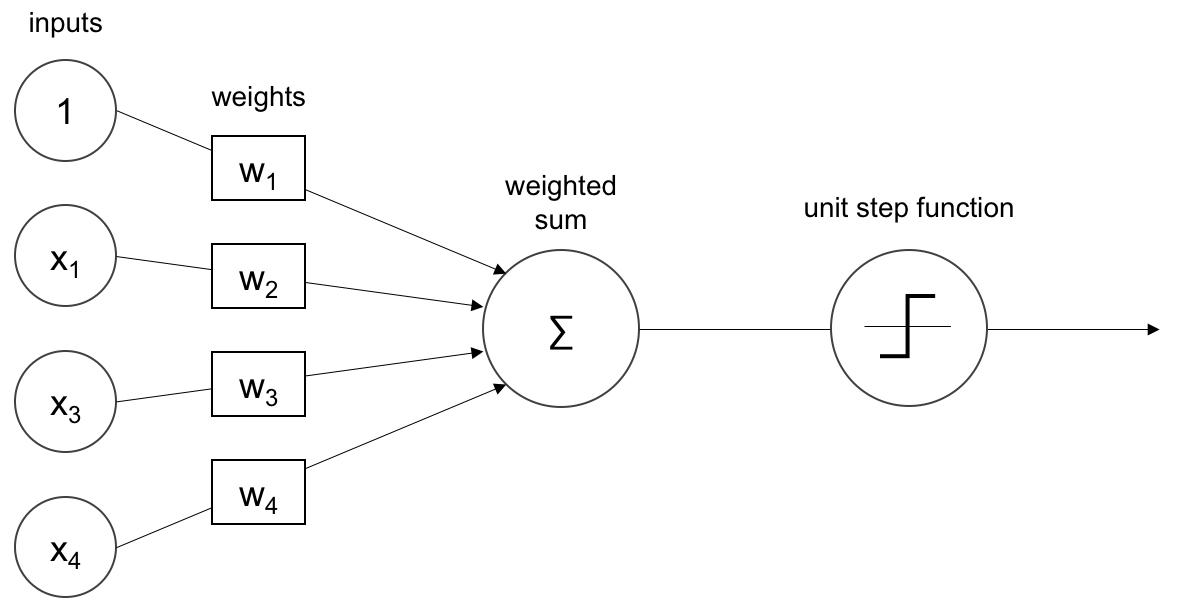
\includegraphics[width=0.6\textwidth]{image3.png}
\caption{The perceptron}
\label{fig:pic3}
\end{figure}

 The weighted sum is passed through a non-linear function called \textit{activation function} to capture the non-linearities in the input.  An \textit{activation function} decides whether a neuron should fire or not. There are various activation functions as shown in \ref{fig:act}. Sigmoid is useful for converting any value to probabilities and can be used for binary classification. The tanh maps input to a value in the range of -1 to 1 and are more stable than sigmoid. The ReLU maps input x to max (0, x) and works well for a large range of problems.
 
\begin{figure}[h]
    \subfigure[Sigmoid function]{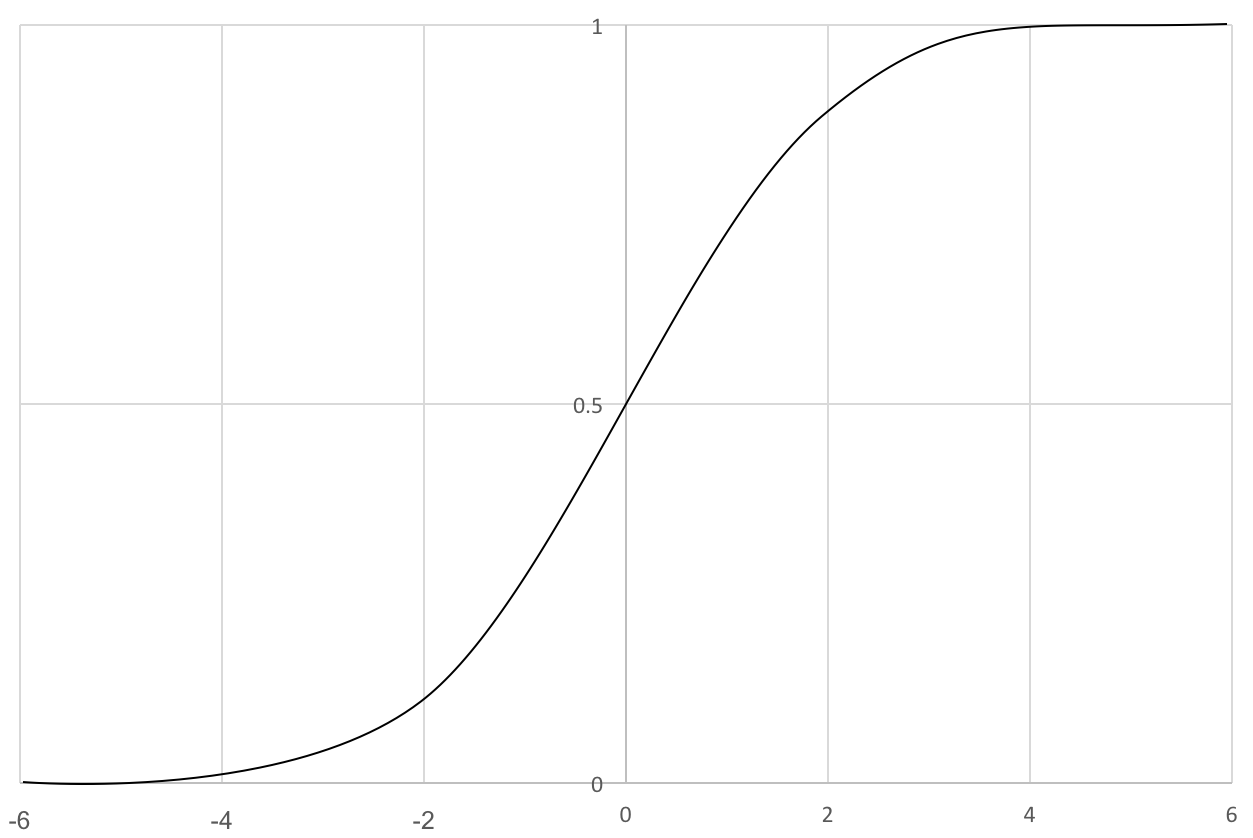
\includegraphics[width=0.30\textwidth]{image4} \label{fig:pic4}}
    \subfigure[Tanh function]{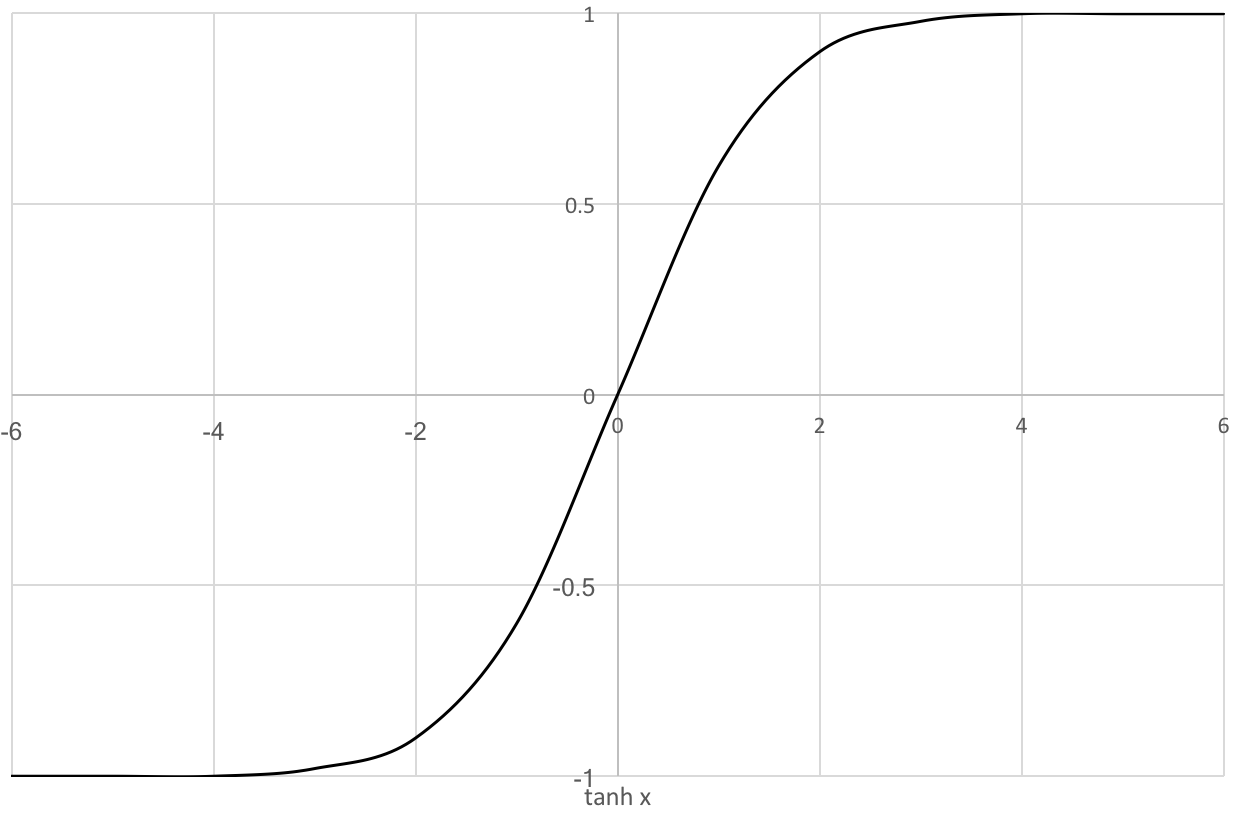
\includegraphics[width=0.30\textwidth]{image5}\label{fig:pic5}}
    \subfigure[RELU function]{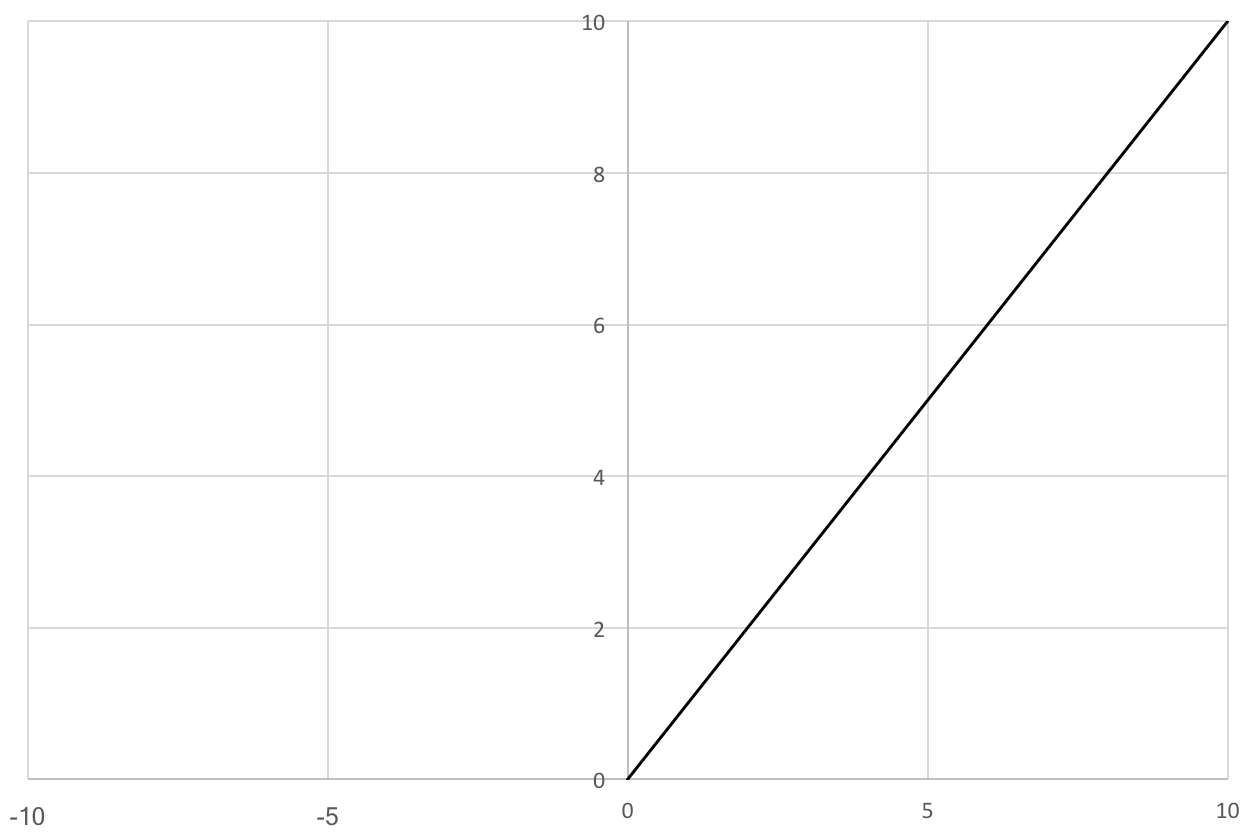
\includegraphics[width=0.30\textwidth]{image6}\label{fig:pic6}}
\caption{Some common activation functions}
\label{fig:act}
\end{figure}


 

\section{Artificial Neural Networks}

The artificial neural network is a collection of perceptrons and activation functions. The perceptrons are connected to each other to form the hidden layers as shown in \ref{fig:pic7}. The training process determines the values of these weights and biases. The training is started by initialising the weights and biases. The error is computed by taking the difference of the actual output to the ground truth. Based on the loss, the weights and biases are tuned in steps. The training is stopped when the error cannot be minimised anymore and during this point, the model is said to learn the features in the input.


\begin{figure}[h]
\centering
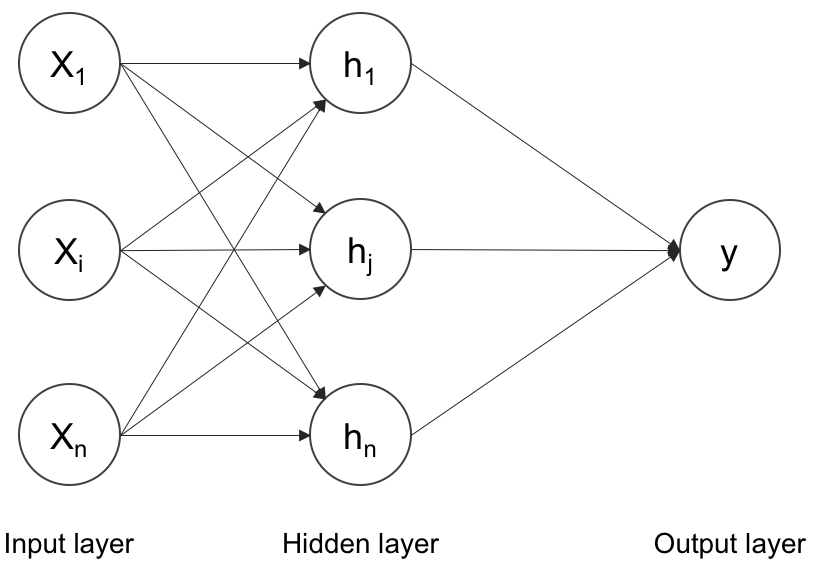
\includegraphics[width=0.6\textwidth]{image7.png}
\caption{Artificial Neural Network}
\label{fig:pic7}
\end{figure}


\section{Training the neural network}

\subsection{Backpropagation}

One of the commonly used algorithms for training the neural networks is the backpropagation algorithm. The weights are updated from the last layer based on the error that is calculated between ground truth and actual output. The error is propagated through the layers until the first layer and at each step the gradients are calculated. The weights are updated using the gradient descent algorithm which is explained in the following section.

\subsection{Gradient Descent}

Often in machine learning, finding the best model for a certain situation means to minimise the error of the model or maximise the likelihood of the data. Hence it can be seen as finding the solution for an optimisation problem. Gradient descent is one of the optimisation problems which is widely used in the algorithms of machine learning and deep learning. 

\subsubsection{Idea}

Suppose we have some function \textbf{f(x)} that takes as input a vector of real numbers and outputs a single real number. One such simple function is given in equation \ref{gradient}. 

\begin{equation} \label{gradient}
f(x) = x^2  \in R
\end{equation}

The \textit{gradient} of \textbf{f(x)} gives the input direction in which the function \textbf{f(x)} most quickly increases. One approach to maximising a function is to pick a random starting point, compute the gradient, take a small step in the direction of the gradient, and repeat with the new starting point. Similarly, we can try to minimise a function by taking small steps in the opposite direction, as shown in \ref{fig:pic0}. 

\begin{figure}[h]
\centering
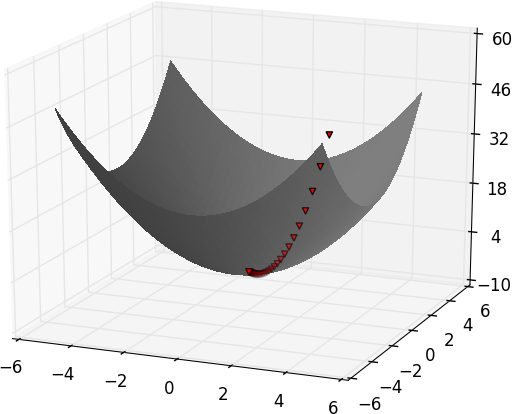
\includegraphics[width=0.6\textwidth]{image1.png}
\caption{Finding a minimum using gradient descent}
\label{fig:pic0}
\end{figure}

This procedure will work very well if the function has a unique global minimum. If a function has multiple (local) minima, this procedure might find the wrong one of them, in which case we might re-run the procedure from a variety of starting points. If a function has no minimum, then it is possible the procedure might go on forever.

\subsubsection{Estimating the gradient}


If f is a function of one variable, its derivative at a point x measures how f(x) changes when we make a very small change to x. The derivative is the slope of the tangent line at (x, f(x)). The gradient can be estimated as given in \ref{eqn:2} by considering h to be very small.

\begin{equation} \label{eqn:2}
Gradient = \frac{f(x+h) - f(x)}{h}
\end{equation}

If f is a function of multiple variables then it has multiple partial derivatives each indicating the change in f when we make small changes to one of the input variables by holding the other variables constant. The learning rate $\eta$ determines the size of the steps we take to reach a (local) minimum. There are three variants of gradient descent as explained in the following sections.

\section{Types of gradient descents }

\subsection{Batch gradient descent}

Batch gradient descent or vanilla gradient descent calculates the gradient of the cost function w.r.t the parameters $\theta$ for the entire training dataset. 

\begin{equation} \label{eqn:3}
\theta = \theta - \eta \cdot \Delta_{\theta} J(\theta)
\end{equation}

Batch gradient descent is slow since we need to calculate the gradients for the whole dataset to make just one update of the parameters. Batch gradient descent is guaranteed to converge to the global minimum for convex error surfaces and to a local minimum for non-convex surfaces.

\subsection{Stochastic gradient descent}

Stochastic gradient descent (SGD) performs parameter update for each training sample. Batch gradient descent performs redundant computations for large gradients since it recomputes the gradients for similar examples before each update. SGD does not have this problem since it performs one update for each training data and is much faster. These frequent updates cause the objective function to fluctuate which may lead to overshooting. However, by setting the optimal learning rate, SGD can show the same behaviour as the batch gradient descent.

\begin{equation} \label{eqn:4}
\theta = \theta - \eta \cdot \Delta_{\theta} J(\theta; x^{(i)}; y^{(i)})
\end{equation}


\subsection{Mini-batch gradient descent}

Mini-batch gradient descent takes the best of SGD and batch gradient descent. It updates the parameters for every mini-batch of \textit{n} training samples. It reduces the variance of the parameter updates and hence more stable convergence. It also makes computations more efficient. 

\begin{equation} \label{eqn:5}
\theta = \theta - \eta \cdot \Delta_{\theta} J(\theta; x^{(i:i+n)}; y^{(i:i+n)})
\end{equation}


\subsubsection{Challenges of mini-batch gradient descent}

\begin{itemize}
	\item Finding the optimum learning rate is difficult. A learning rate which is too small will take lots of time to converge and a learning rate too fast might overshoot and oscillate around the minimum.
	\item Neural networks usually have highly non-convex error functions with saddle points. These are the points where one dimension slopes up and other slopes down. The SGD finds these points very hard to escape since the gradient is close to zero in all dimensions.
\end{itemize}

\chapter{Deep learning}

Conventional machine-learning techniques were unable to process natural data in their raw form. For decades, pattern-recognition systems needed carefully engineered features extracted from raw data to be fed into the learning systems such as classifiers. \textit{Representation learning} is a set of methods that allows a machine to be fed with raw data and to automatically discover the representations needed for detection or classification \cite{lecun2015deep}. \textit{Deep learning} methods are representation-learning methods with multiple levels of representation, obtained by composing simple non-linear modules that each transform the representation at one level into a representation at a higher and more abstract level \cite{lecun2015deep}. An example of deep learning can be multiple layer feed forward neural network with non-linear activations. With enough transformations, any complex function can be learned.  This is known as the \textit{universal approximation theorem} \cite{csaji2001approximation}.


\section{Artificial intelligence and Deep Neural Networks}

 Deep neural networks (DNNs) form a part of broad field of Artifical intelligence (AI). DNNs are currently the foundation of many AI applications\cite{lecun2015deep}. The number of applications using deep neural networks(DNNs) have increased tremendously since they were applied successfully to speech recognition \cite{Deng2013RecentAI}, image recognition \cite{Krizhevsky2012ImageNetCW}, etc. However, there is a trade-off between the accuracy of DNNs and the cost of high computational compexity. Hence, graphics processing units (GPUs) are widely used for training and inference of deep neural networks. 

\section{Convolutional Neural Networks}

The convolutional neural networks (CNNs) are considered one of the most promising solutions for various computer vision tasks such as object detection \cite{ren2015faster}, image recognition, etc. CNNs were first introduced through the work of LeCuN in 1989 \cite{lecun1989backpropagation} for processing handwritten zip codes. The success of CNNs has attracted attention from companies such as Google, Microsoft, AT\&T, Facebook etc., \cite{khan2019survey}. The architecture of CNN consists of multiple learning stages composed of a combination of convolutional layer, non-linear processing units and subsampling layers. Each layer generates higher level abstractions called a \textit{feature map}. The regular neural networks do not scale to full images since they have fully connected layers at the input. For example, an image of 240*480*3 would lead to neurons that have 240*480*3 weights. This would lead to a huge number of parameters and hence to overfitting. In a convolutional neural network, the neurons in a layer will only be connected to a small region of the layer before it, instead of a fully connected network. A convNet is made up of layers and each layer transforms an input 3D volume to an output 3D volume with some differentiable function. 



\begin{figure}[h]
\centering
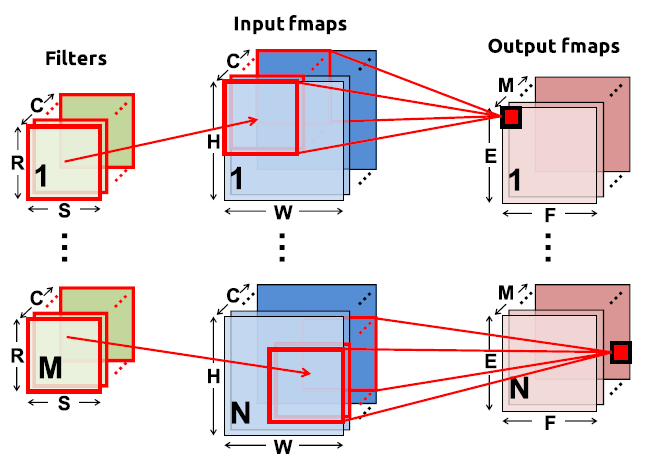
\includegraphics[width=1\textwidth]{cnn.png}
\caption{Convolution operation in CNN \cite{sze2017efficient}}
\label{cnn}
\end{figure}


\subsection{Convolution layers}

Each of the convolution layer in CNNs is composed of convolutions as shown in figure \ref{cnn}. The weighted sum for each output activation is computed using only a small neighbourhood of input activations. This neighbourhood is known as \textit{filter size}. The size of the ouput feature map depends on the number of filter kernels used, the padding and the stride of convolution operation. The computation of the convolution layer can be defined as below equation \ref{eqn1} \cite{sze2017efficient}

\begin{equation} \label{eqn1}
O[z][u][x][y] = B[u] + \sum_{k=1}^{C-1}\sum_{i=1}^{S-1}\sum_{j=1}^{R-1} I[z][k][U_{x}+i][U_{y}+j] * W[u][k][i][j]
\end{equation}

\[0 \leq z < N ,0 \leq u < M,0 \leq x < F,0 \leq y < E\]

\[E = \frac{H - R + U}{U}, F = \frac{W - S + U}{U}\]  
\newline
where, 
\newline
O = output feature map matrix
\newline
I = input feature map matrix
\newline
W = filter matrix 
\newline
B = bias matrix
\newline
N = batch size
\newline
M = number filters
\newline
H, W, C = input feature map dimensions
\newline
R, S, C = filter dimensions
\newline
E, F, M = output feature map dimensions
\newline 
U = stride size

\subsection{Pooling layer}

Pooling is the group of computations that reduce the dimensions of the feature maps. Pooling enables the network to be invariant to small shifts and distortions. The most common pooling operations are max pooling and average pooling where usually stride size of 2 or greater is used. 


%https://ujjwalkarn.me/2016/08/11/intuitive-explanation-convnets/




\section{Semantic Segmentation}

Semantic segmentation is understanding an image at the pixel level. In this task, each pixel is assigned a label which tells us which object the pixel belongs to. It is a high-level task that leads us towards complete scene understanding. There are many approaches to solving the problem of semantic segmentation in computer vision literature. The popularity of deep learning and convolutional neural network has influenced the problem of semantic segmentation as well \cite{zhu2016beyond}. These techniques of deep learning and CNNs surpass other approaches by a large margin in terms of accuracy and efficiency\cite{zhao2017survey}. The operation is similar to convolution but instead of multiplying with the filter kernel, sampling is done by either taking the maximum or average of the values of the feature map matrix in the neighbourhood of the filter size. 


\begin{figure}[h]
\centering
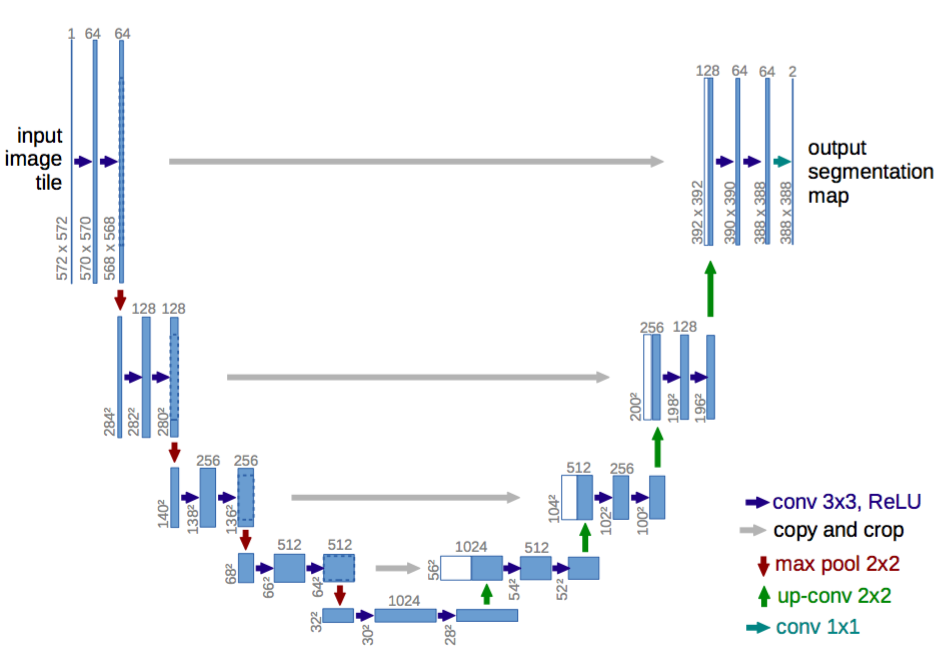
\includegraphics[width=1\textwidth]{unet.png}
\caption{U-net: Encoder-decoder architecture \cite{ronneberger2015u}}
\label{unet}
\end{figure}


\subsubsection{Different approaches to semantic segmentation}

Before deep learning, there were methods like TextonForest\cite{shotton2008semantic} and Random Forest based classifiers for semantic segmentation. One of the popular initial deep learning approaches was patch classification \cite{ciresan2012deep} where a patch of the image around a pixel was used to classify each pixel into classes. In recent years, convolutional neural networks have had enormous success on segmentation problems. In 2014, a CNN method for solving segmentation called Fully Convolutional Networks \cite{long2015fully} was introduced. It was a dense prediction method without any fully connected layers. This meant that segmentation maps of any size could be generated and was also much faster compared to the patch classification approach. All the subsequent variants of semantic segmentation are based on this approach. The other problem apart from using fully connected layers in CNNs for segmentation is pooling layers. Pooling layers introduce the property of \textit{spatial invariance} to the network whereby it discards the 'where information'. However, the semantic segmentation problem needs this 'where information' to predict the class maps for the pixels. Two different classes of literature evolved to solve this problem. 


\subsubsection{Encoder - Decoder architecture}
First one is the encoder-decoder architecture. The idea is that the encoder gradually reduces the spatial dimensions with pooling layers and the decoder gradually recovers the object details and spatial dimensions. There are shortcut connections from the encoder to decoder help the decoder in recovering the object details as shown in \ref{unet}. U-net \cite{ronneberger2015u} belongs to this class of architecture. The key idea of fully convolutional networks\cite{long2015fully} is that the fully connected layers in the classification networks can be viewed as convolutions with kernels that cover their entire input regions. After convolutionalizing the fully connected layers in a imagenet pretrained network like VGG, the feature maps needs to be upsampled because of the pooling operation of VGG network. This upsampling is done by \textit{deconvolutional layers}. But, upsampling with deconvolutional layers produces coarse segmentation maps because of the loss of information during pooling. Therefore skip connections are introduced from higher resolution feature maps. 


\begin{figure}[h]
\centering
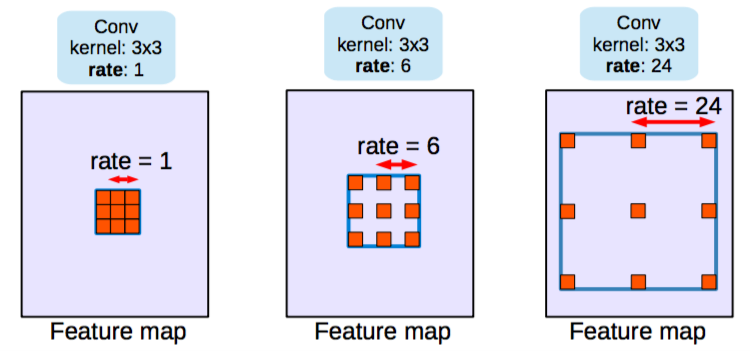
\includegraphics[width=1\textwidth]{dilated_conv.png}
\caption{Dilated/atrous convolutions \cite{yu2015multi}}
\label{dilated}
\end{figure}


\subsubsection{Dilated/Atrous convolutions}
The second type of architectures are called as dilated/atrous convolutions and they do not include the pooling layers. Dilated convolutional layer allows for an exponential increase in field of view without decrease of spatial dimensions. It can be thought of the reverse process of convolution where the spatial dimensions increase as shown in \ref{dilated}. 


\section{Transfer learning}

Deep learning networks are \textit{data dependent}. The scale of the model and the size of the data is linearly dependent. Many domains face the problem of insufficient training data. Often the model faces situations where it has not seen the data before and does not know how to deal with it. In all of such situations the current state-of-the-art models either show degraded performance or even break down. Transfer learning can help us deal with such scenarios.

Transfer learning allows us to use the already existing labelled data of some related task or domain. The name transfer learning is derived from the fact that we try to transfer as much knowledge as we can from the source to our target task or domain. 

\subsection{Definition}

As per the definition in \cite{pan2010survey}, transfer learning involves a domain and a task. A domain \textbf{D} consists of a feature space \textbf{X} and a marginal probability distribution \textbf{P(X)} over the feature space. Given a domain, \textbf{D = (X, P(X))}, a task \textbf{T} consists of a label space \textbf{Y} and a conditional probability distribution \textbf{P(Y$\vert$X)} that is learnt from the training data. Given a source domain \textbf{D$_{s}$} and a corresponding source task \textbf{T$_{s}$} as well as a target domain \textbf{D$_{t}$} and a target task \textbf{T$_{t}$}, the objective of transfer learning is to enable to learn the target probability distribution \textbf{P(Yt$\vert$Xt)} in \textbf{D$_{t}$} with the information gained from \textbf{D$_{s}$} and \textbf{T$_{s}$} where  \textbf{D$_{s}$} $\neq$ \textbf{D$_{t}$} or \textbf{T$_{s}$} $\neq$ \textbf{T$_{t}$}. 

Given source and target domains \textbf{D$_{s}$} and \textbf{D$_{t}$} where \textbf{D = (X, P(X))} and source and target tasks \textbf{ts} and \textbf{T$_{t}$} where \textbf{T = (Y, P(Y$\vert$X))} there can be four transfer learning scenarios.

\begin{enumerate}
	\item \textbf{Xs} $\neq$ \textbf{Xt}. The feature space of source and target domain are different. 
	\item \textbf{P(Xs)} $\neq$ \textbf{P(Xt)}. Marginal probability distributions of source and target domain are different.
	\item \textbf{Ys} $\neq$ \textbf{Yt}. The label spaces between the two tasks are different.
	\item \textbf{P(Ys$\vert$Xs)} $\neq$ \textbf{P(Yt$\vert$Xt)}. The  conditional probability distributions of the source and target tasks are different.
\end{enumerate}
%Pan, S. J., & Yang, Q. (2010). A survey on transfer learning. IEEE Transactions on Knowledge and Data Engineering, 22(10), 1345–1359.

\subsection{Transfer learning methods}

Transfer learning has been investigated in the past \cite{pan2010survey}. With the approach of deep learning, there are new methods of transfer learning available.
%Razavian, A. S., Azizpour, H., Sullivan, J., & Carlsson, S. (2014). CNN features off-the-shelf: An astounding baseline for recognition. IEEE Computer Society Conference on Computer Vision and Pattern Recognition Workshops, 512–519.
The most common way of applying transfer learning for a given problem is by using pretrained features. It is also the method which has been used in this project. The lower layers of the convolutional neural networks capture the low-level image features such as edges, corners etc., while the higher convolutional layers capture more and more complex details such as body parts, faces etc. The final fully connected layers are assumed to capture information that is relevant to solving the respective task, for example, the classes in case of the classification task.
Thus we can simply use the features of a state-of-the-art network such as ENet\cite{Paszke2017ENetAD} pre-trained on Cityscapes dataset \cite{Cordts2016Cityscapes} and train a new model on these extracted features. In practice, we keep the earlier layers of the network fixed or tune them with very low learning rate so as to not unlearn these features. This simple approach has been shown to achieve great results on various computer vision tasks \cite{pan2010survey}.

%\begin{figure}[h]
%\centering
%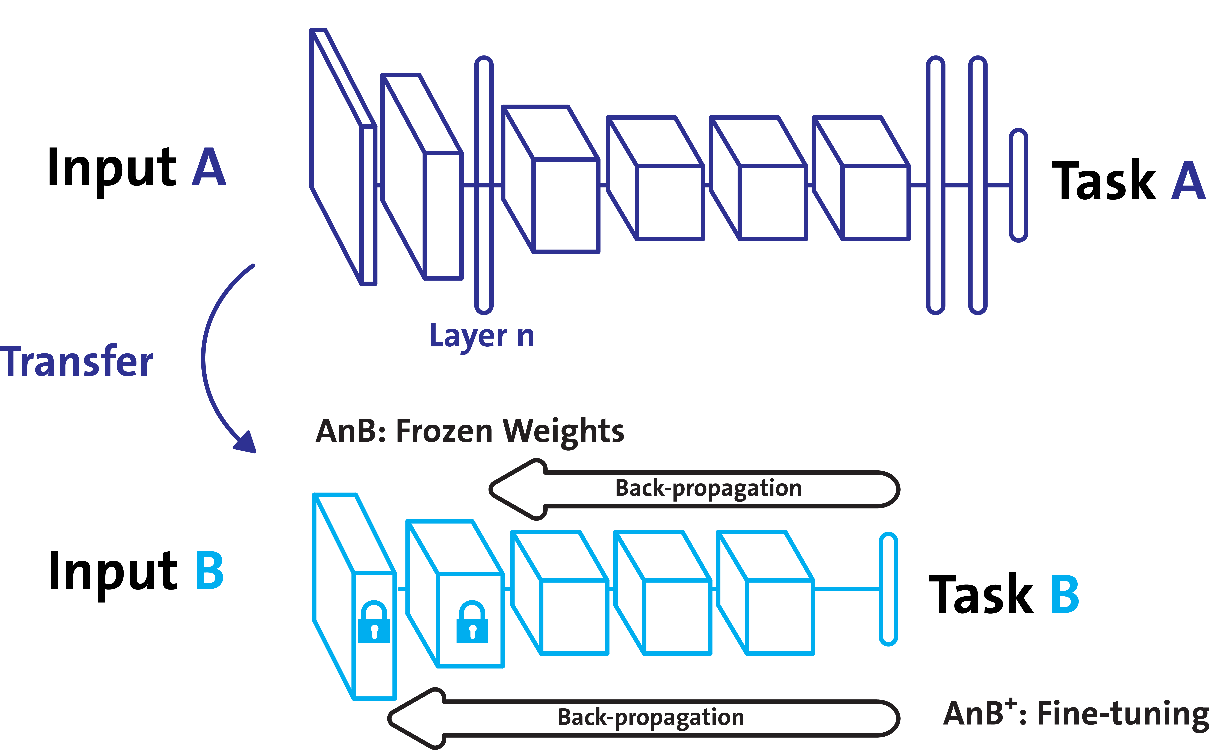
\includegraphics[width=0.75\textwidth]{transferlearning.png}
%\caption{Transfer Learning source = www.oreilly.com}
%\label{transferlearning}
%\end{figure}

\chapter{Method}

The aim of the project is to detect free space in a given image taken by a fisheye camera in an autonomous car. Free space is defined as the region in the image, where no other object is visible and the projection lies on the ground plane. The project has been divided into three sub-tasks as below

\begin{enumerate}
	\item To create a dataset of annotated fisheye images of road scenes.
	\item To use the created dataset to train a neural network.
	\item To use this neural network to detect free space in test images.
\end{enumerate}

\begin{figure}[h]
\centering
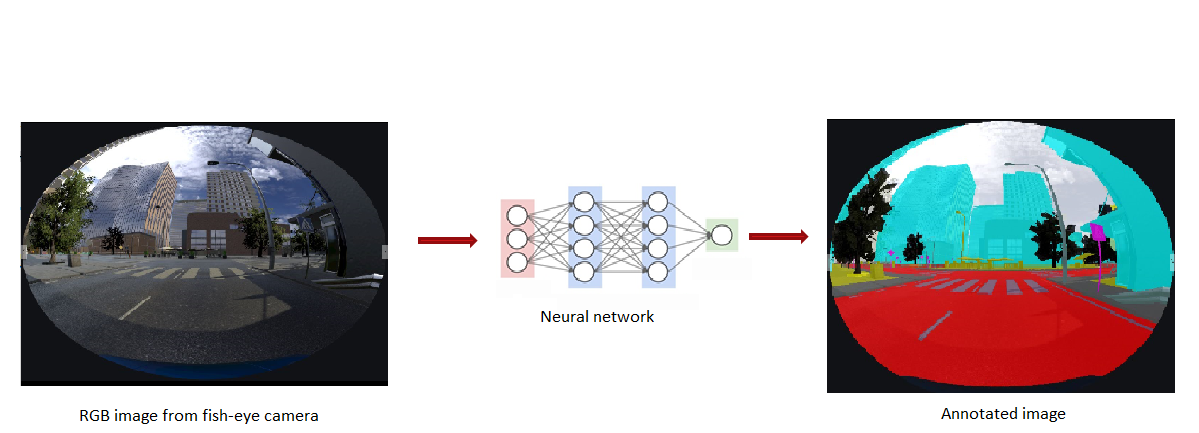
\includegraphics[width=1\textwidth]{fisheyesegment.png}
\caption{Fisheye image segmentation}
\label{fisheyesegment}
\end{figure}

\section{Dataset generation}

There is no publicly-available annotated fisheye image dataset of road scenes. Hence in this project, simulated images and labels are generated using Unity software framework \cite{unity3d}. The advantage of using simulation is that the labels are implicitly created when an object is created inside the simulation. Unity provides free environments for development. One of the city environments which looks realistic and can be used for free is Windridge city. It has buildings, city props, road, lane markings, countryside, trees etc., (figure \ref{windridge}) which can be used for image and label generation.

\begin{figure}[h]
\centering
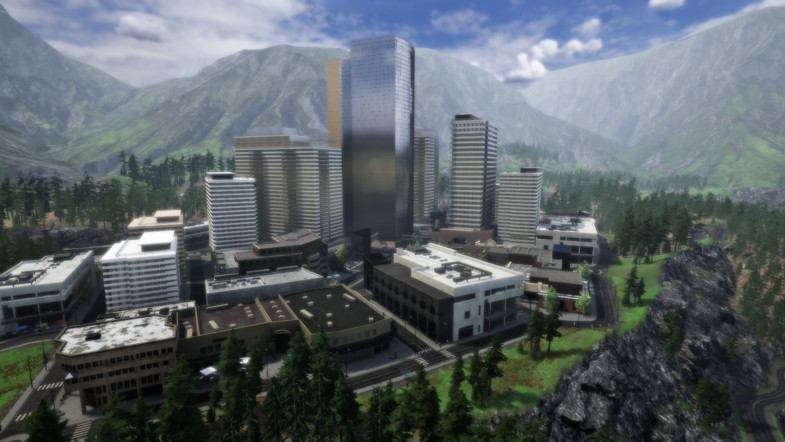
\includegraphics[width=1\textwidth]{windridge.jpg}
\caption{Windridge city in Unity}
\label{windridge}
\end{figure}
 

We now need a car which has all the physics properties such as collision body, gravity etc., to roam around the windridge city, collecting images and labels. For this purpose, there is a framework from Microsoft known as Microsoft Airsim \cite{airsim2017fsr}. Airsim is a simulator for cars and drones and is built on Unreal Engine. It is open-source, cross-platform and it supports hardware-in-loop for realistic simulations. Microsoft has recently released Airsim plugin for Unity. Airsim also exposes APIs to retrieve data from the car such as steering angle, acceleration and also APIs to control the car through the code. 

For the purposes of this project, the dataset generation step can be further split into the following steps.

\begin{enumerate}
	\item To set up Unity software with Windridge environment and Airsim plugin.
	\item To project the images of the simulation as fish-eye projections.
	\item To store the images and label by driving around the simulation environment.
\end{enumerate}

\subsection{Unity Airsim setup with Windridge environment} \label{instructions}

The installation described here is for Windows 10 x64 machine with Nvidia Quadro M2200 graphics card. For this project Unity 2018.3.2f1 version was used. For linux installations, please visit the respective websites of Unity and Airsim.  Once the software is downloaded and installed, we need to install the Airsim plugin for unity. 


\begin{figure}[h]
\centering
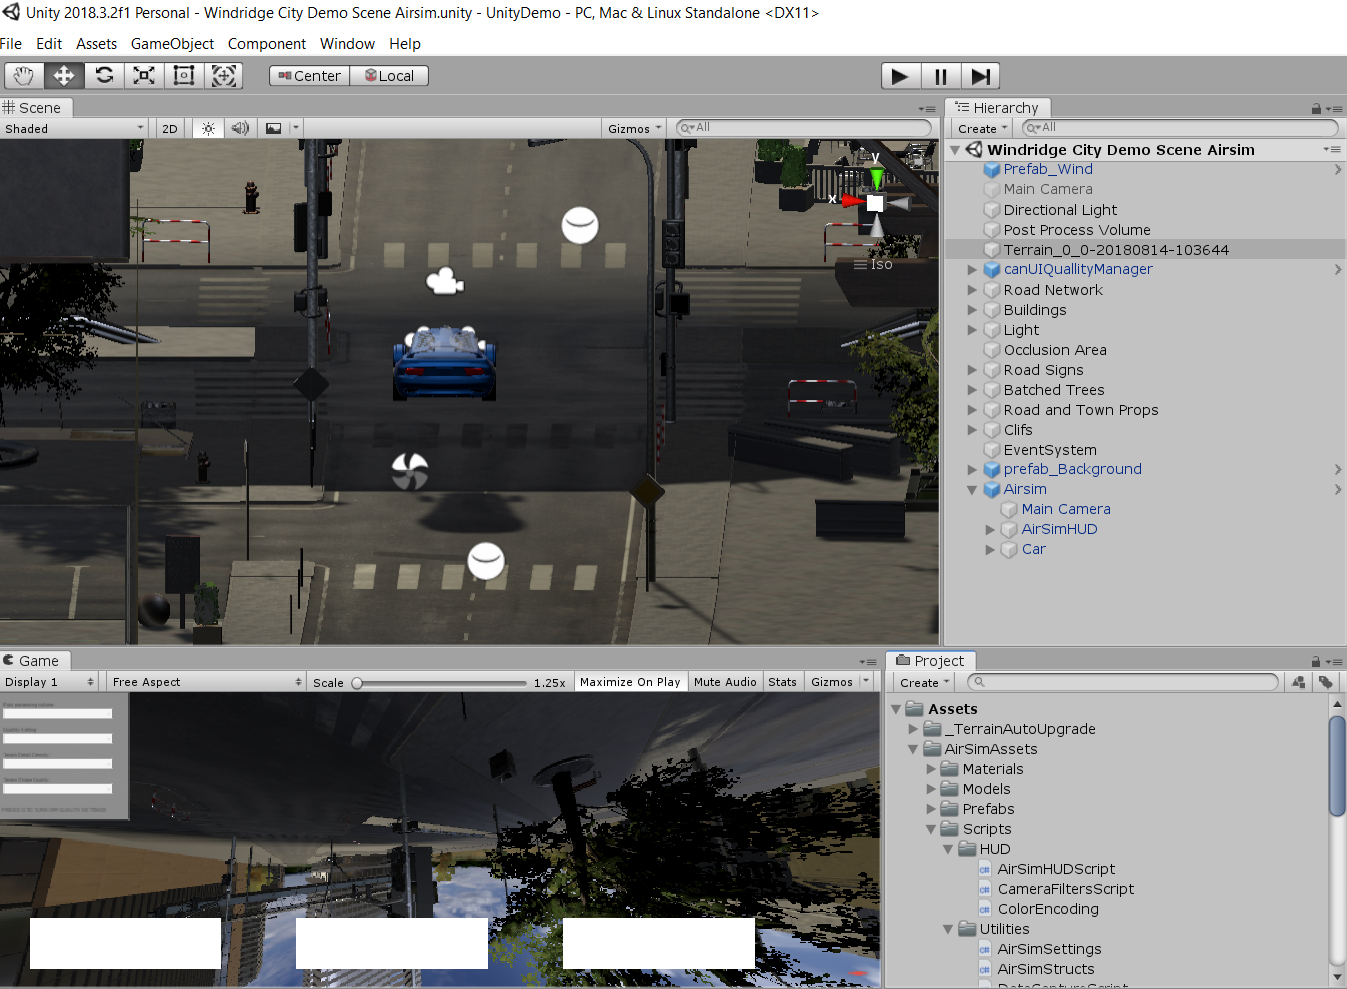
\includegraphics[width=1\textwidth]{WindridgeScene.png}
\caption{Windridge Scene with Airsim assets}
\label{windridgescene}
\end{figure}


\begin{enumerate}
	\item Download the unity editor from the Unity website\cite{unity3d}.
	\item Install Visual Studio 2017 and clone the git repo https://github.com/Microsoft/AirSim.git
	\item Run build.cmd from the command line. 
	\item Now build the unity project by running build.cmd inside Unity folder of the git repo.
	\item Create a new Unity project and download Windridge city asset inside it from the unity asset store.
	\item From the UnityDemo/Assets folder of the above git repo, copy the folders AirSimAssets, Plugins and Standard Assets into the Assets folder of your new Unity project.
	\item From the UnityDemo/Assets/Scenes folder of the git repo, copy CarDemo.unity into the Assets/Scenes folder of your new Unity project.
        \item Copy "AirsimHUD", "Car", "Main Camera" items from CarDemo scene into the Windridge City Demo Scene.
	\item Change the position of the Car and Main Camera to that of the Main Camera of the Windridge scene.
	\item Remove the old Windride camera. Make sure the new camera has Smooth flow script with Target as "LookAt"
	\item The final scene should look as in figure \ref{windridgescene}
\end{enumerate}

The unity project used for this research work can be found at https://git.dst.etit.tu-chemnitz.de/admal/fisheyeroad.

\subsection{Fisheye image projection in Unity}

In fisheye projections, straight lines do not appear straight. The camera in the Airsim Car is a pin-hole camera which can give depth and segmented views. Since we need fisheye projection we need to modify the code and assets in the Unity environmnet. Unity provides a standard perspective projection with at most 120-degree field of view (FOV). Also, this limited FOV has distortion and pixel inefficiency. The solution is to render multiple perspective views and combine these together to form the required FOV \cite{bourke2009idome}.

\begin{figure}[h]
\centering
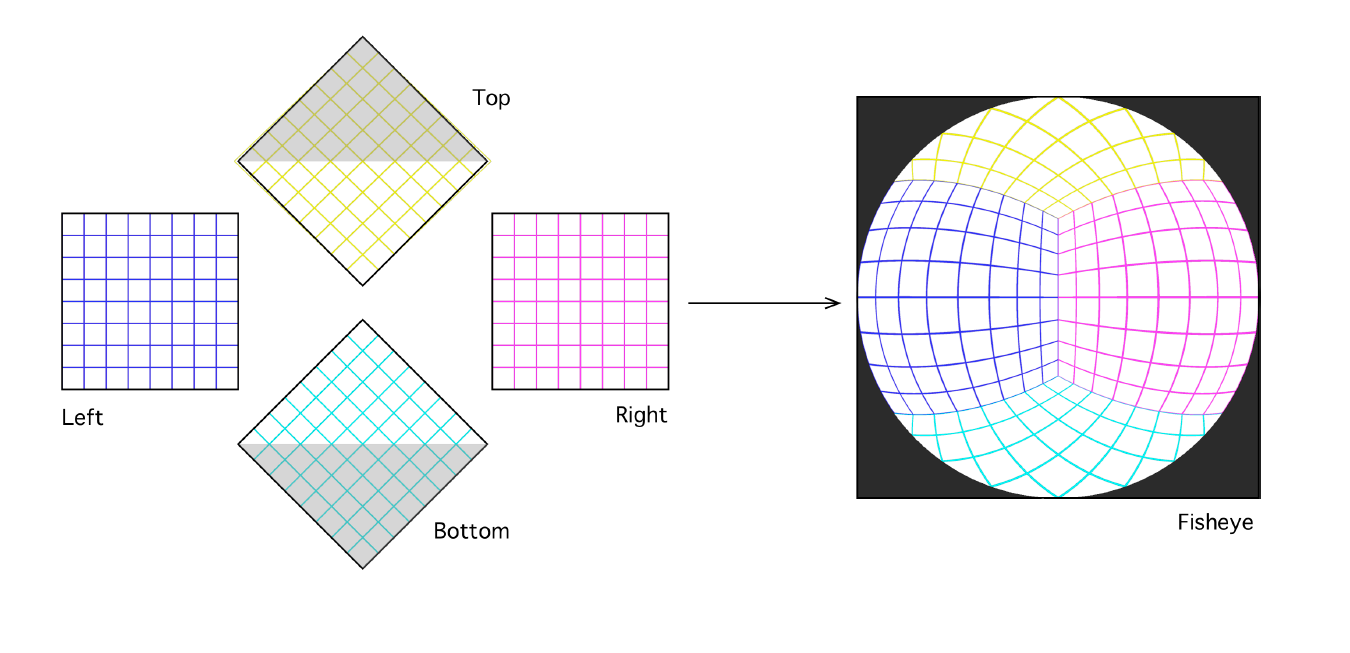
\includegraphics[width=1\textwidth]{fisheyestitch.png}
\caption{Flow diagram of the 5 pass rendering algorithm. 4 passes create the fisheye projection and an additional pass creates the geometry corrected fisheye \cite{bourke2009idome}}
\label{fisheyestitch}
\end{figure}

According to the author in  \cite{bourke2009idome}, there are two ways to do this. One is to create a vertex shader that pre-distorts the geometry of the world in such a way that the distorted geometry when viewed with an orthographic camera results in fisheye projection. But this technique is computationally expensive especially when there are multiple polygons and meshes in the scene, since a polygon may need to be drawn differently depending on both its distance and angle to the camera. 

The other solution and the one used in this project is to render multiple views and to stitch those together to form a fisheye projection. Four views each of standard perspective projection of FOV 90 degrees are taken as shown in \ref{fisheyestitch}. These 4 renders are applied as textures to one of the 4 meshes whose texture coordinates are designed such that the final projection results in fisheye projection.






\subsection{Implementation of fisheye projection with Airsim}

As mentioned in \ref{instructions}, once the Windridge City environment is ready with Airsim plugin, we need to create the fisheye projection. For this we add four cameras: top, bottom, left and right, each of which renders to the four render textures which is then applied to the 4 meshes of fisheye projection. The next step is to render depth and  segmentation of each of the four cameras and render to the fisheye projection. For this, four render passes are created in Unity which renders the depth and segmented view separately to the render textures of the fisheye projection as shown in figure \ref{render}. The car can now be driven around with the keys W,S,A,D and with the help of Unity function EncodeToPNG(), the fish-eye projection with the depth and the segmented layer data can be stored on the disk. We also extract the mapping of the semantic layer color to the class it belongs through a json file. New classes can be added by defining new layers and assigning the corresponding asset to the layer.

\begin{figure}[h] 
    \subfigure[Fish-eye projection]{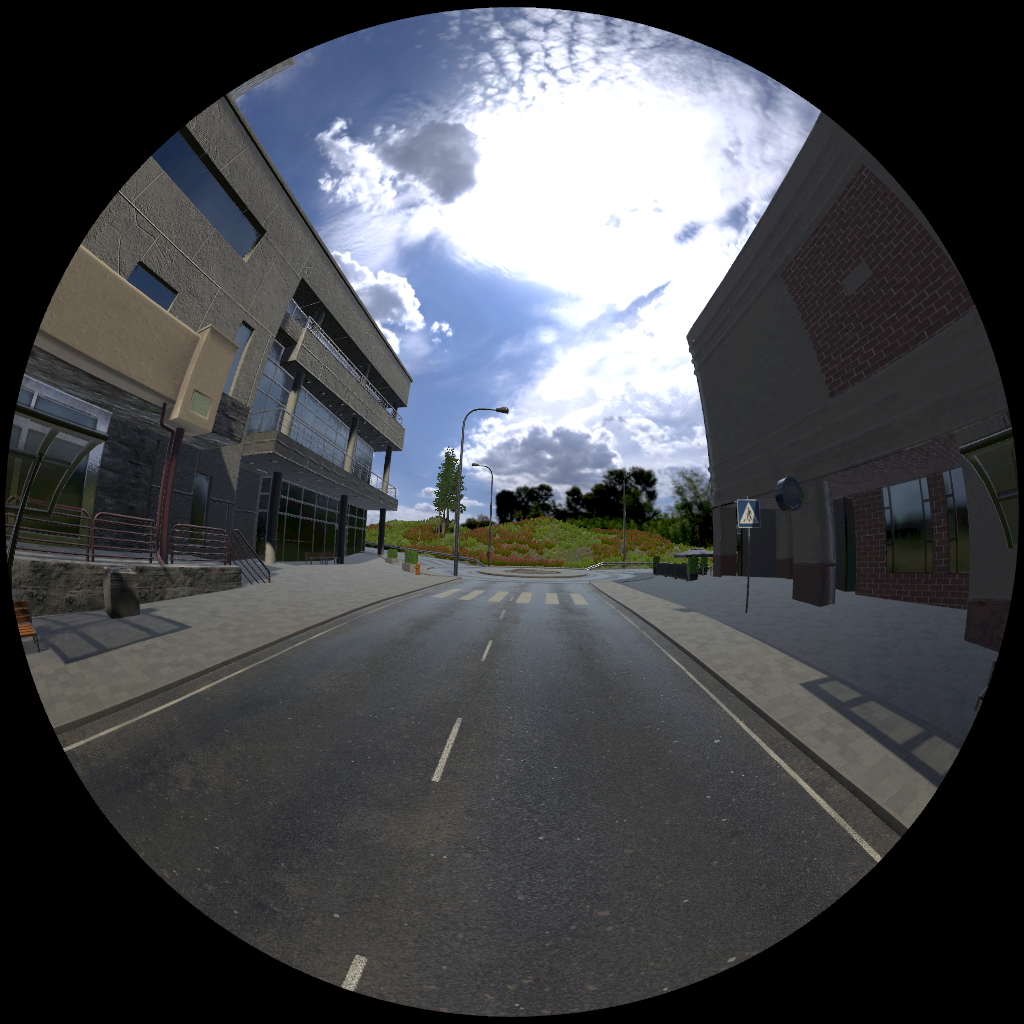
\includegraphics[width=0.3\textwidth]{0000004_img.png} \label{imageview}}
    \subfigure[Fish-eye projection with depth]{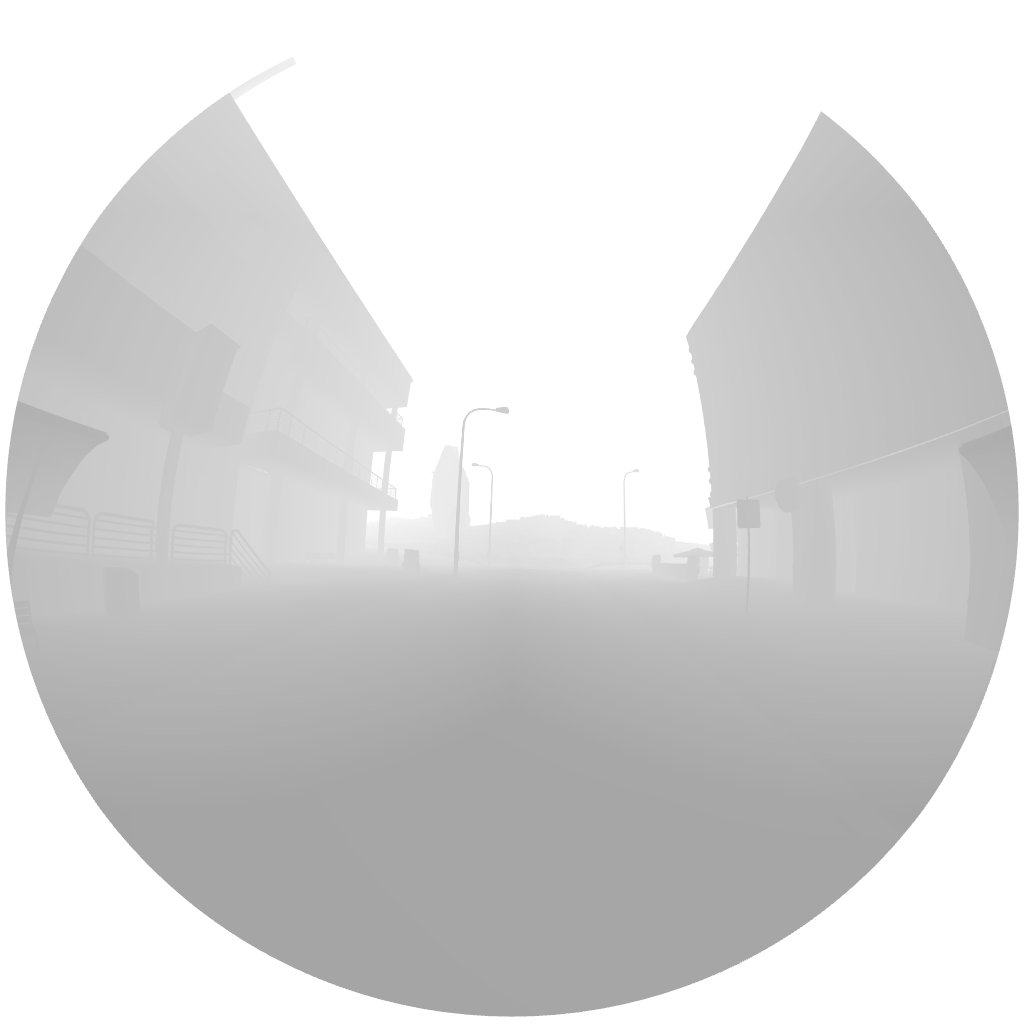
\includegraphics[width=0.3\textwidth]{0000004_depth.png}\label{depthview}}
    \subfigure[Fish-eye projection with segmentation]{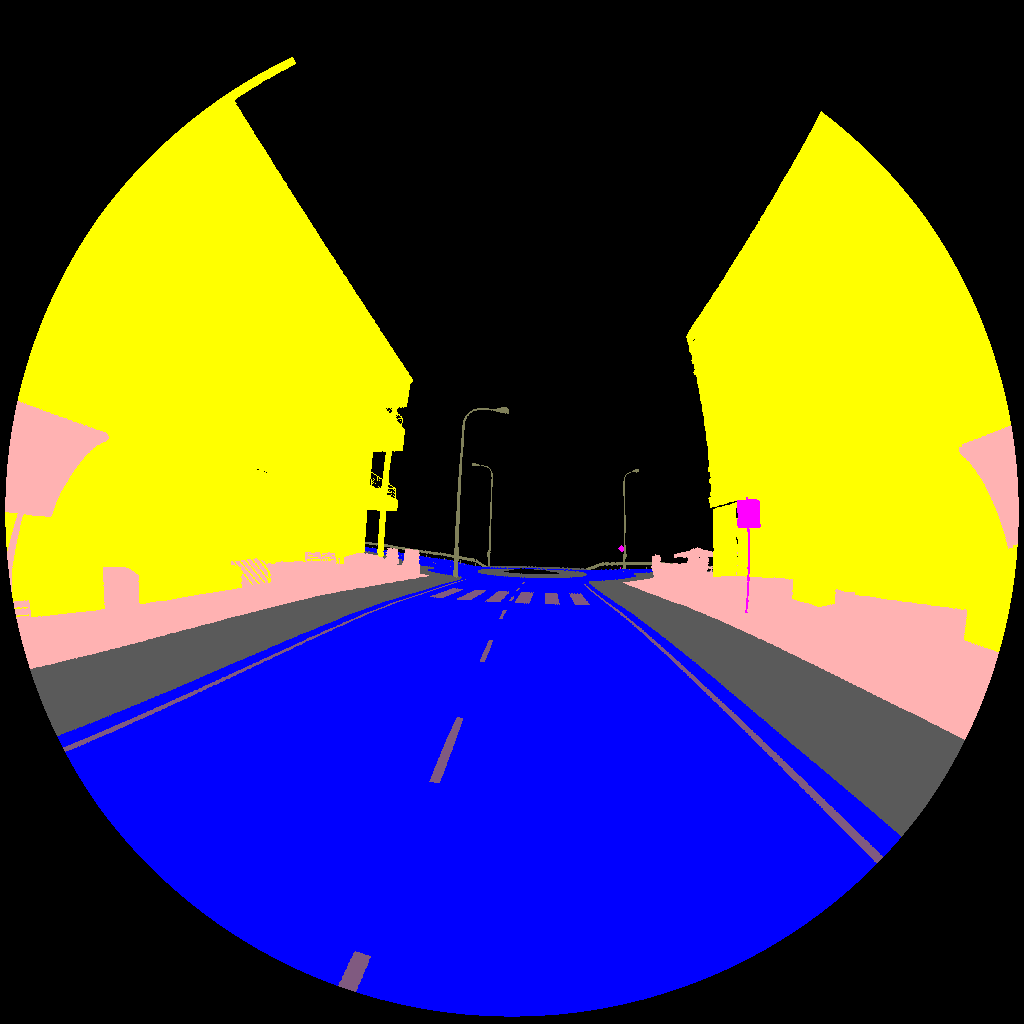
\includegraphics[width=0.3\textwidth]{0000004_layer.png}\label{semanticview}}
\caption{Fish-projection in Unity using 4 cameras and 3 render passes} \label{render}
\end{figure}



\section{Preprocessing the data}

Using the method mentioned in the previous sections, around 2500 images are generated, which are then divided into train, test and validation in the ratio of 80:10:10. The extracted images are having RGB intensities which need to be mapped to the class labels. This is done with the help of Tensorflow functions. The images are then augmented by flipping them and hence creating a dataset with around 5000 images. These images are then used to perform transfer learning on pre-trained E-Net model as explained in the next sections. The classes which are used in the project are listed in table \ref{classtable}. The problem is then converted to a binary classification problem by assigning Road, footpath and lane marking classes as free space and others as not free space. 



% % Example of, how to use a Table

\blindtext[1]

\begin{center}
\begin{tabular}{|c|c|c|c|}
\hline
Research study & Objective & Features & Classifier\\
\hline
Driver Gaze Zone Estimation using Convolutional Neural Networks:
A General Framework and Ablative Analysis & 80& 0.3153 & 0.4900\\
500 & 120& 0.1229& 0.1787\\
1000 & 120& 0.0680& 0.0880\\
2000 & 120& 0.0361& 0.0441\\
5000 & 140& 0.0256& 0.0305\\
5000 & 164& 0.0343& 0.0880\\
\hline
\end{tabular}
\captionof{table}{This is the caption of the table}
\label{tab:table1}
\end{center}

\blindtext[3] % Load Data from File example_tables
\begin{center}
\captionof{table}{Class number to pixel intensity mapping}
\label{classtable}
\begin{tabular}{| l | l | l | l |}
\hline
Class number & Class name & RGB color & Free space\\
\hline
0 & Background & [21, 18, 17] & 0\\
\hline
1 & Road & [0, 0, 255] & 1\\
\hline
2 & Buildings & [255, 255, 0] & 0\\
\hline
3 & Road Signs & [255, 0, 255] & 0\\
\hline
4 & Trees & [0, 255, 255] & 0\\
\hline
5 & Road and town props & [0, 178, 178] & 0\\
\hline
6 & Cliffs & [178, 255, 178] & 0\\
\hline
7 & Vehicle & [128, 128, 128] & 0\\
\hline
8 & Footpath & [90, 90, 90] & 1\\
\hline
9 & Road post & [128, 128, 90] & 0\\
\hline
10 & Lane Marking & [128, 90, 128] & 1\\
\hline
11 & Road curb & [90, 128, 128] & 0\\
\hline
12 & Traffic Lights & [128, 90, 0] & 0\\
\hline
13 & Low pixels & [0, 0, 0] & 0\\
\hline
14 & High pixels & [255, 255, 255] & 0\\
\hline
\end{tabular}

\end{center}


\newpage

\section{Model}

In autonomous vehicles, predicting free space at real time is very important. Deep neural networks for semantic segmentation have the disadvantage of requiring a large number of floating point operations and long run-times. ENet (efficient neural network) \cite{Paszke2017ENetAD} is used for tasks requiring low latency operations. The authors claim that the network is up to 18x faster, requires 75x less FLOPs, has 79x less parameters and provides similar or better accuracy to existing models\cite{Paszke2017ENetAD}. This network is used as the base model for the transfer learning in our project.



%\begin{figure}[h]
%\centering
%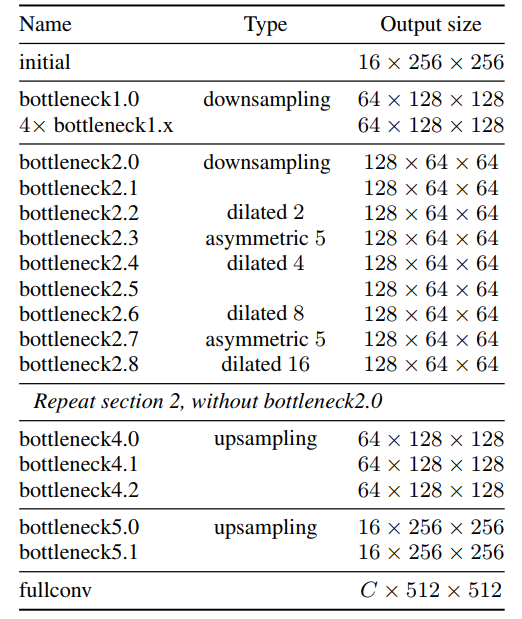
\includegraphics[width=0.5\textwidth]{Enet.png}
%\caption{E-net architecture\cite{Paszke2017ENetAD}}
%\label{enet}
%\end{figure}

\subsection{Network architecture}

The network architecture is as shown in table \ref{enet}. The network is divided into several stages as highlighted by the horizontal lines in the table and the first digit after each block name. Output sizes in the table are for an input image of size 512*1024. The initial block is represented as shown in \ref{initial} and the bottleneck is represented as shown in \ref{bottleneck}.  

\begin{figure}[h]
    \subfigure[Initial Block]{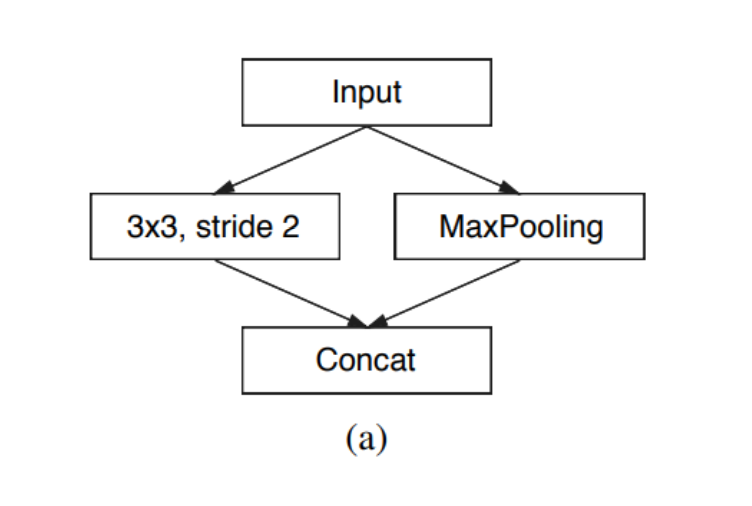
\includegraphics[width=0.49\textwidth]{initialblock.png} \label{initial}}
    \subfigure[Bottleneck block]{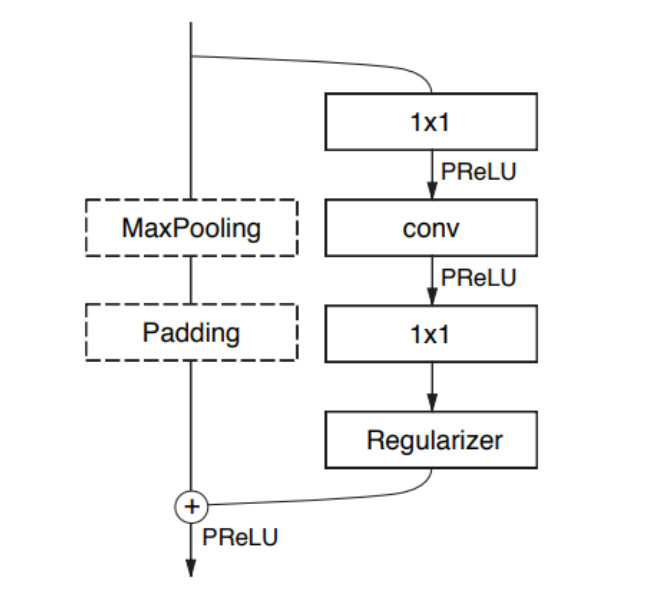
\includegraphics[width=0.37\textwidth]{bottleneck.png}\label{bottleneck}}
\caption{Visual representation of ENet modules  \cite{Paszke2017ENetAD}}
\end{figure}

\subsubsection{Initial block}

The initial block as shown in \ref{initial} consists of a single block. The input image of size 512 * 1024 is fed to the input layer which is then passed through a convolution layer with 13 filters each of size 3*3*3. A bias vector of size 13 and convolution strides of [1,2,2,1] are used. Thus an output feature map of size 256*512*13 is obtained. Then, a maxpooling operation with a kernel size of [1, 2, 2, 1] and strides of [1, 2, 2, 1] is performed on the input image which gives an output feature map of size 256*512*3. These two feature maps are concantenated to obtain a final output feature map of size 256*512*16. Finally, batch normalization and PReLU activation are computed on the output feature map. The weights for convolution filter are initialized with Xavier initializer\cite{glorot2010understanding} and zero padding is used.  

\subsubsection{Bottleneck module}

The bottleneck module is as shown in \ref{bottleneck}.The features of the bottleneck module are summarised as below.

\begin{itemize}
	\item Each block consists of three convolution layers: 1*1 projection that reduces the dimensionality, a main convolution layer and a 1*1 expansion. 
	\item Batch Normalization  \cite{ioffe2015batch} and PReLU \cite{he2015delving} are added between all convolutional layers
	\item If the bottleneck is downsampling, a max pooling layer is added to the main branch. Also, the first convolution is replaced with 2*2 convolution with stride of 2 in both dimensions. Then the output is zero padded to match the size of required output feature map.
	\item The main convolution ('conv' in \ref{bottleneck}) is either regular, dilated or full convolution with 3*3 filters. Sometimes, it is asymmetric convolution with a sequence of 5*1 and 1*5 convolutions. 
	\item Regularizer is Spatial Dropout \cite{tompson2015efficient} with $\rho$=0.01 before bottleneck 2.0 and $\rho$=0.1 afterwards.
	\item Bias terms are not used for 1*1 projection and expansion to reduce the number of kernel calls. 
	\item In the decoder,as shown in dotted lines in \ref{bottleneck}, max pooling is replaced with max unpooling and padding is replaced with spatial convolution without bias. Also, decoder uses ReLU instead of PReLU and no regularizer.
\end{itemize}

The network architecture as shown in table \ref{enet} is composed of an initial block followed by successive bottleneck modules. The network can be thus divided into seven layers: initial block, bottleneck 1-5 and a fully-connected layer. The layers 2-4 can be considered as encoder layers and layers 5-6 as decoder layers. The fully convolution layers at the end takes most of the processing time of the decoder.

\begin{center}
\captionof{table}{Network architecture}
\label{enet}
\begin{tabular}{| l | l | l |}
\hline
Name & Type & Output size\\
\hline
initial &  & 256*512*16\\
\hline
bottleneck 1.0 & downsampling & 128*256*64\\
bottleneck 1.1 & downsampling & 128*256*64\\
bottleneck 1.2 & downsampling & 128*256*64\\
bottleneck 1.3 & downsampling & 128*256*64\\
bottleneck 1.4 & downsampling & 128*256*64\\
\hline
bottleneck 2.0 & downsampling & 64*128*128\\
bottleneck 2.1 & downsampling & 64*128*128\\
bottleneck 2.2 & dilated 2 & 64*128*128\\
bottleneck 2.3 & asymmetric 5 & 64*128*128\\
bottleneck 2.4 & dilated 4 & 64*128*128\\
bottleneck 2.5 &   & 64*128*128\\
bottleneck 2.6 & dilated 8   & 64*128*128\\
bottleneck 2.7 & asymmetric 5   & 64*128*128\\
bottleneck 2.8 & dilated 16   & 64*128*128\\
\hline
bottleneck 3.1 &   & 64*128*128\\
bottleneck 3.2 & dilated 2 & 64*128*128\\
bottleneck 3.3 & asymmetric 5 & 64*128*128\\
bottleneck 3.4 & dilated 4 & 64*128*128\\
bottleneck 3.5 &  & 64*128*128\\ 
bottleneck 3.6 & dilated 8 & 64*128*128\\
bottleneck 3.7 & asymmetric 5 & 64*128*128\\
bottleneck 3.8 & dilated 16 & 64*128*128\\
\hline
bottleneck 4.0 & upsampling  & 128*256*64\\ 
bottleneck 4.1 &   & 128*256*64\\ 
bottleneck 4.2 &   & 128*256*64\\ 
\hline
bottleneck 5.0 & upsampling & 256*512*16\\ 
bottleneck 5.1 &   & 256*512*16\\
\hline
fullconv & & 512*1024*16\\
\hline
\end{tabular}
\end{center}



\subsection{Transfer learning using tensorflow}

The dataset generated using Unity is trained on pretrained E-net model \cite{Paszke2017ENetAD}. The model is selected on the basis of the author's claim that it performs well in real time. Pretrained E-net model which was trained on Cityscapes dataset \cite{Cordts2016Cityscapes} for 23 epochs was taken as the starting point in the model design. The fully convolution layer of the E-Net model is modified with outputs as a tensor of size 15 corresponding to the 15 classes of our dataset. The model is then trained for 100 epochs with the same hyperparameters as the original model.
\newline

\begin{enumerate}
\item The pre-trained model is first restored using the below code.

\begin{lstlisting}
saver = tf.train.Saver(tf.trainable_variables()[:-2])
saver.restore(sess, "./model_1_epoch_23.ckpt")
\end{lstlisting}

\item The tensor before the fully-connected layer is retreived.
\begin{lstlisting}
layer5 = model.graph.get_tensor_by_name("Relu_81:0")
\end{lstlisting}

\item Flow of gradients to intial layers can be stopped using the below code. This is an optional step. In our project this is not done so that the entire network is trained with weights initialized from pretrined E-Net.

\begin{lstlisting}
layer5 = tf.stop_gradient(layer5)
\end{lstlisting}

\item A new fully convolution layer is added with the number of neurons as the number of classes.
\end{enumerate}

\subsection{Loss function and training}

\subsubsection{Softmax cross entropy loss}

The loss function used in the project is pixel-wise cross entropy loss which examines each pixel individually, comparing class predictions to one-hot encoded target vector. Since, the cross entropy loss evaluates class predictions for each pixel vector and then averages over all pixels, it is a problem in our case since the classess have unbalanced representation in the image. The solution is to use class weights in the calculation of average loss.

\subsubsection{Class weights}

The authors in \cite{Paszke2017ENetAD} have calculated the class weights for the training dataset by using a custom equation as shown in \ref{eqn3}.


\begin{equation} \label{eqn3}
W_{class} = \frac{1}{ln(c+p_{class})}
\end{equation}

where 

c = 1.02, a hyperparameter, which restricts the class weights in the range [1, 50 ] and 
$p_{class}$ is the class probability of each pixel for the whole training set.


\subsubsection{Weight decay}

To prevent overfitting, L2 regularization is added to the loss function. This is done by calculating the L2 norm of each of the weight and bias tensors and multiplying them with the weight decay factor. The new loss function with L2 regularization is as shown in equation \ref{eqn2}.


\begin{equation} \label{eqn2}
L_{total} = L + \lambda\Vert w \Vert _{2}^2
\end{equation}

These L2 terms are collected for all the weights and biases and are added to the weighted softmax cross entropy loss function.


\subsubsection{Training}

The model is trained using Adam optimizer \cite{kingma2014adam} for a total of 100 epochs. The hyperparameters used for training are listed in table  

\begin{center}
\captionof{table}{Hyperparameters used for training}
\label{enet}
\begin{tabular}{| l | l |}
\hline
Hyperparameter & Value \\
\hline
Learning rate & 0.0005\\
Weight decay & 0.0002\\
Epochs & 100\\
Batch size & 4\\
Keep probability $\rho$ & 0.01, 0.1\\
\hline
\end{tabular}
\end{center}


\chapter{Results}

\section{Training and validation performance of the model}

The results comparing the loss to the number of epochs for both training and validation is as shown in figure \ref{loss}. As seen in the figure, the training and validation loss decrease from a high value to values close to 4.0 This shows that the model is not overfitting the data and has learnt the features well. The model can be further trained by varying the hyperparameters and modifying the architecture, however, these results are enough to demonstrate that a dataset generated from the simulation can be used to train and validate a neural network.

\begin{figure}[h] 
    \subfigure[Training loss vs epochs]{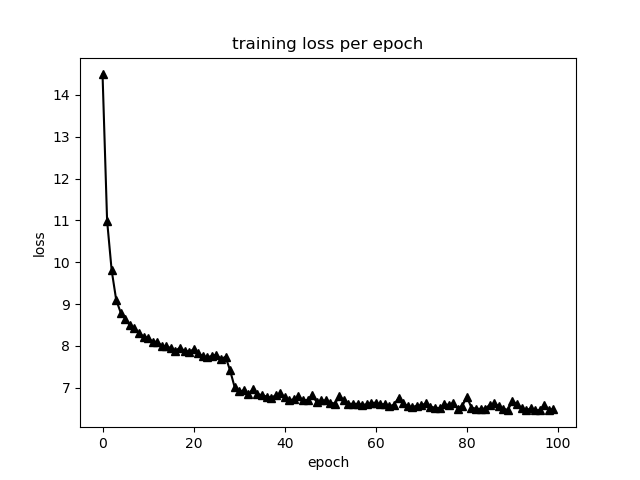
\includegraphics[width=0.5\textwidth]{train_loss_per_epoch.png} \label{trainloss}}
    \subfigure[Validation loss vs epochs]{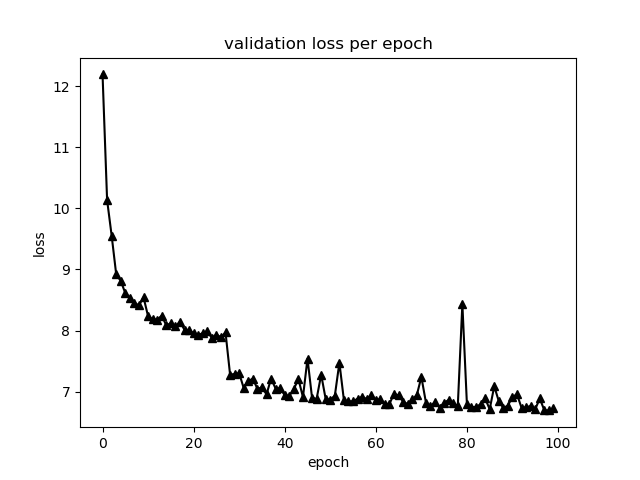
\includegraphics[width=0.5\textwidth]{val_loss_per_epoch.png}\label{valloss}}
\caption{Training and validation losses as compared to the epochs} \label{loss}
\end{figure}

\newpage

\section{Model evaluation on simulated test data}


For evaluating the model, a test set of 141 images was created initially which is used to evaluate after the training. The model predicts 15 classes, however for our purposes, we make the problem binary classification by assigning the labels as free space or not as shown in table \ref{classtable}. The average metrics for pixel accuracy, pixel precision and pixel recall are then calculated and are given in table \ref{resultstable}

\begin{center}
\captionof{table}{Pixel wise results comparison of E-net vs our model on test dataset}
\label{resultstable}
\begin{tabular}{| l | l | l | l |}
\hline
Model & Accuracy & Precision & Recall\\
\hline
E-Net model & 71.2\% & 77.3\% & 56.7\%\\
\hline
Our model & 87.2\%  & 98.5\% & 55\%\\
\hline
\end{tabular}

\end{center}


The images and ground truth are as shown in figure \ref{unityimages} and \ref{unitygt} respectively. The predictions of using our model trained for 100 epochs is as shown in figure \ref{unityp}. The predictions of E-net model are shown in figure \ref{unityp2}. As seen from the figures and from table \ref{resultstable}, our model performs better on fisheye images than the E-net model.

\begin{figure}[h] 
    \subfigure[]{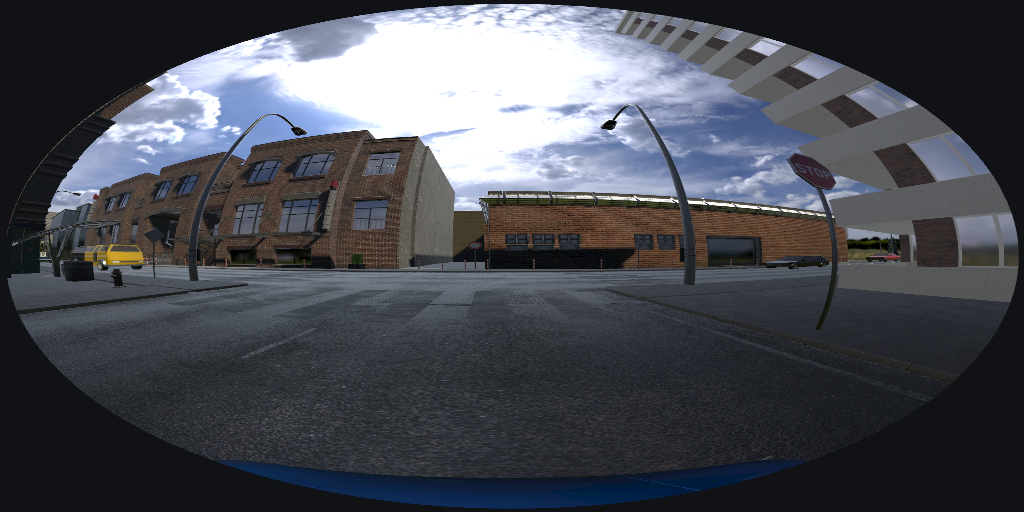
\includegraphics[width=0.3\textwidth]{139_img.png} }
    \subfigure[]{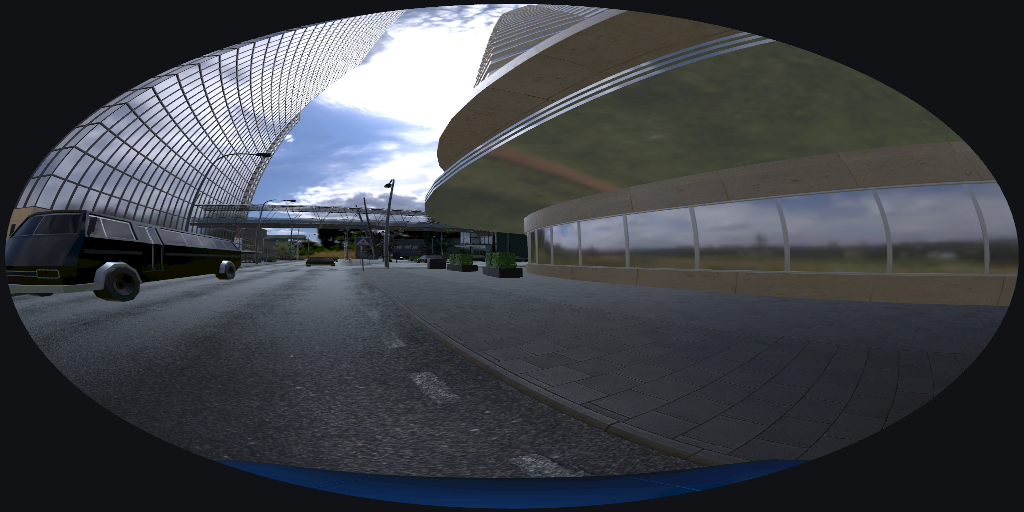
\includegraphics[width=0.3\textwidth]{949_img.png}}
    \subfigure[]{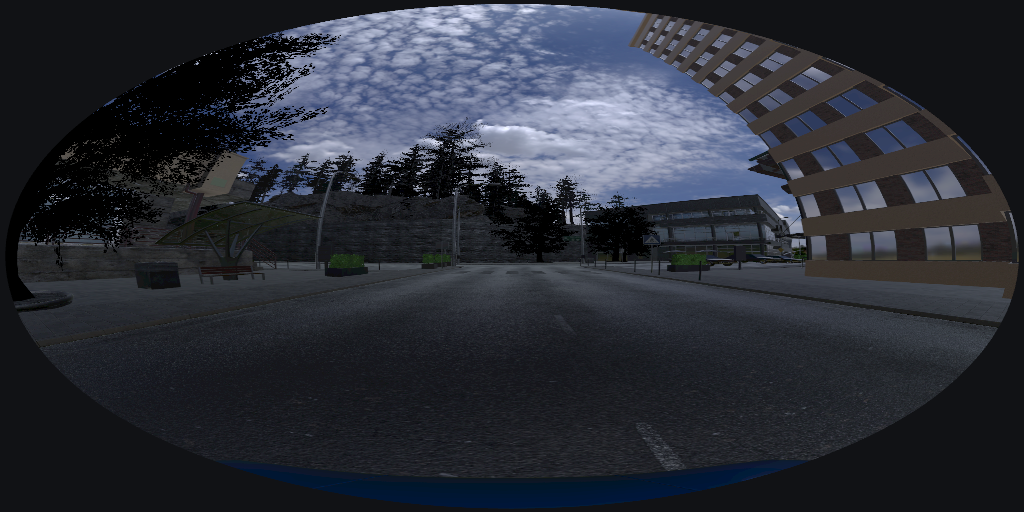
\includegraphics[width=0.3\textwidth]{1296_img.png}}
\caption{Simulated images from unity} \label{unityimages}
\end{figure}

\begin{figure}[h] 
    \subfigure[]{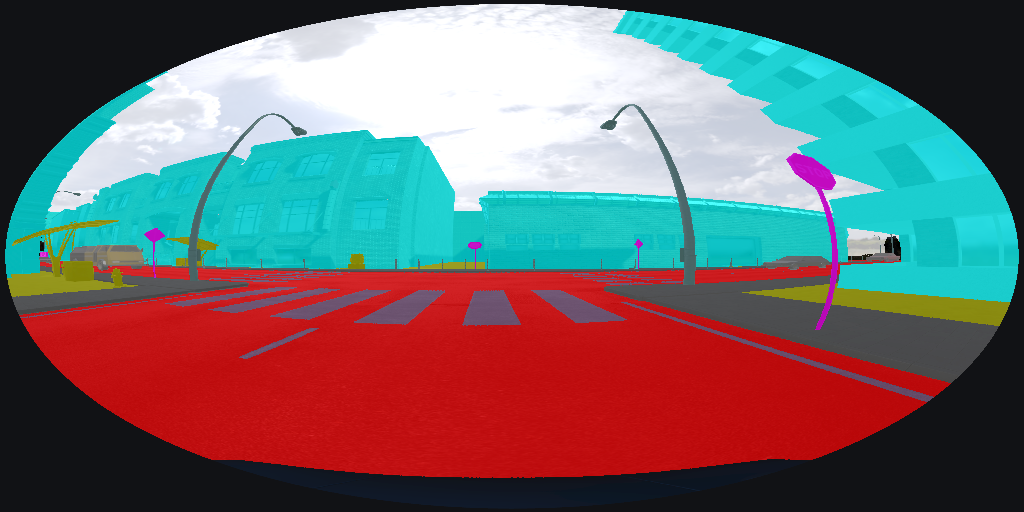
\includegraphics[width=0.3\textwidth]{139_label.png} }
    \subfigure[]{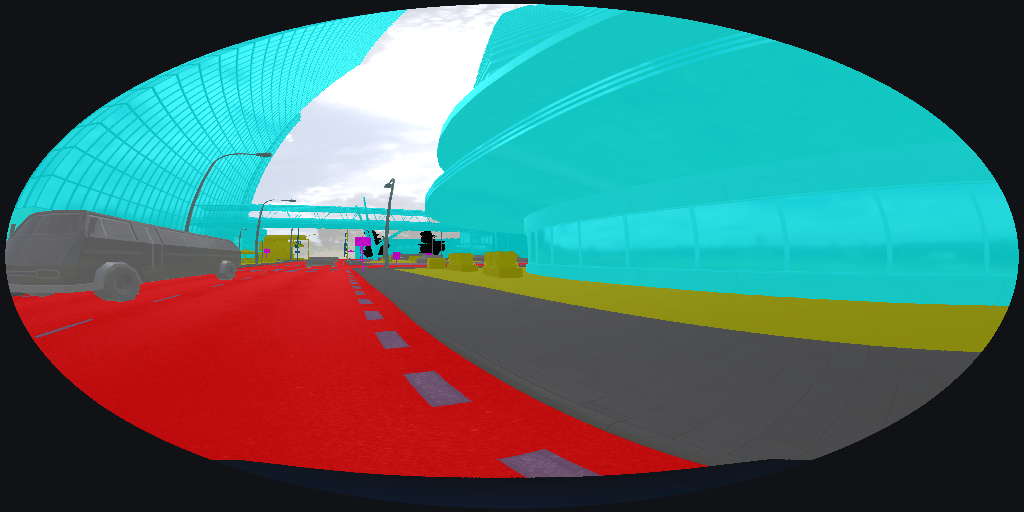
\includegraphics[width=0.3\textwidth]{949_label.png}}
    \subfigure[]{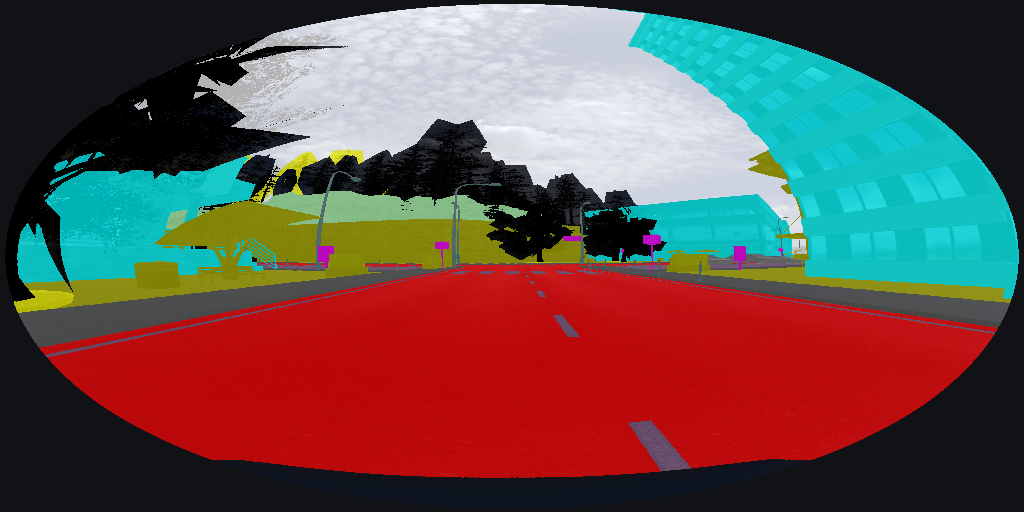
\includegraphics[width=0.3\textwidth]{1296_label.png}}
\caption{Ground truth labels} \label{unitygt}
\end{figure}

\begin{figure}[h] 
    \subfigure[]{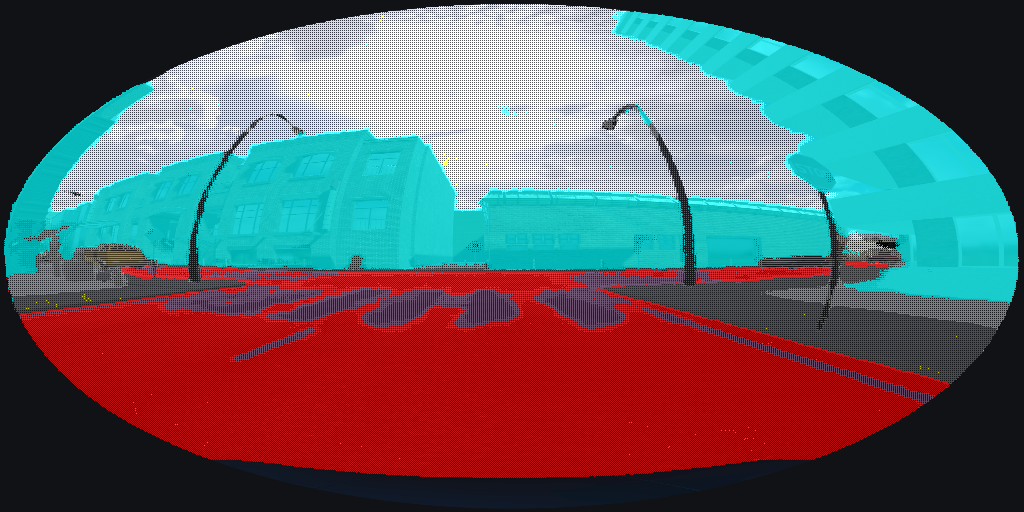
\includegraphics[width=0.3\textwidth]{139_pred.png} }
    \subfigure[]{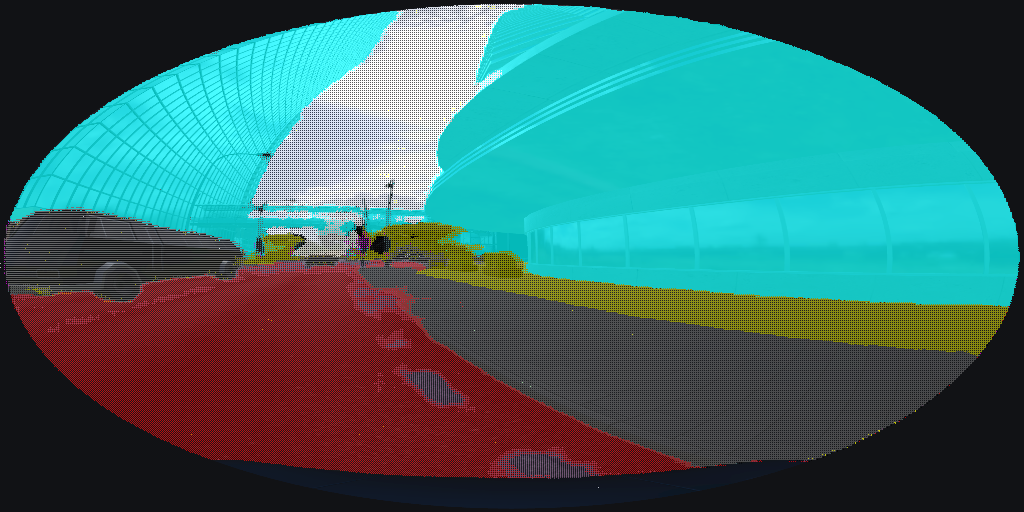
\includegraphics[width=0.3\textwidth]{949_pred.png}}
    \subfigure[]{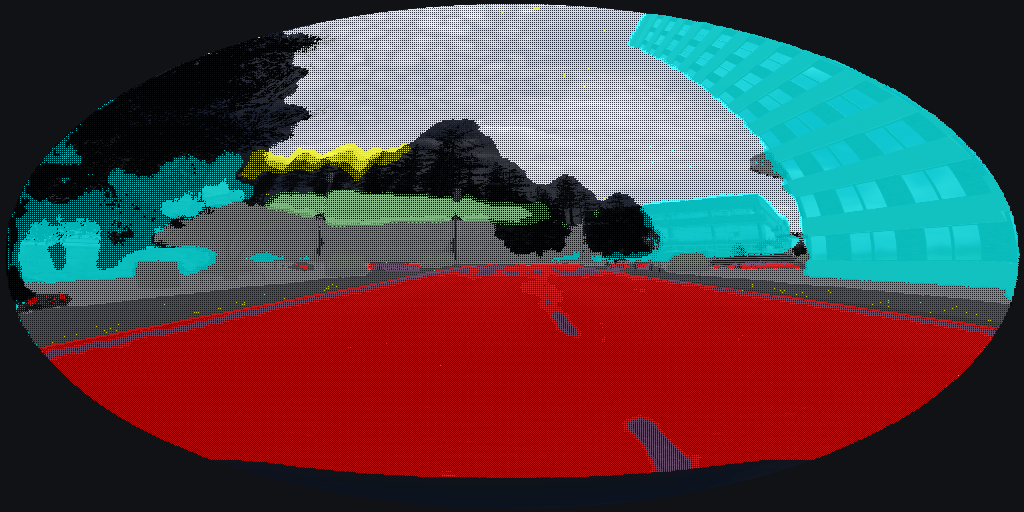
\includegraphics[width=0.3\textwidth]{1296_pred.png}}
\caption{Predicted labels from our model} \label{unityp}
\end{figure}

\begin{figure}[h] 
    \subfigure[]{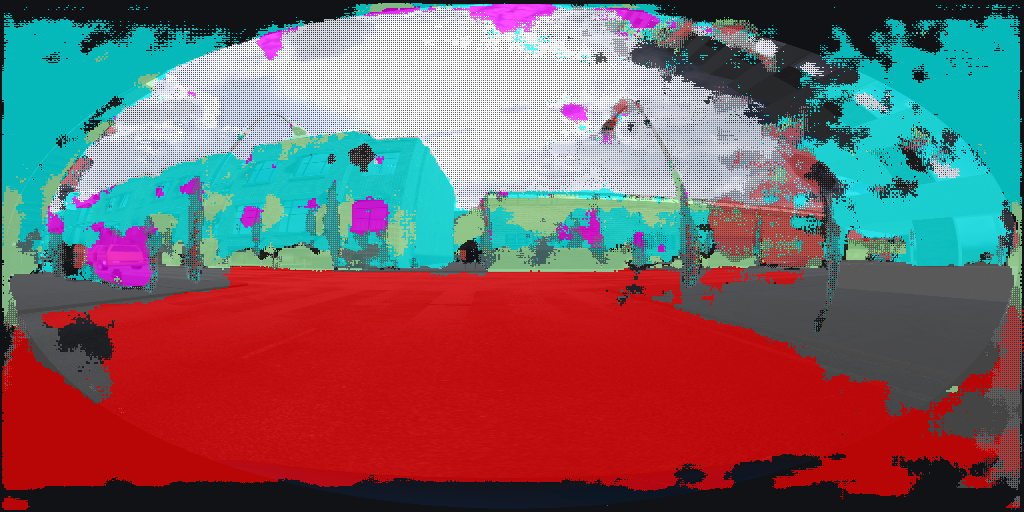
\includegraphics[width=0.3\textwidth]{139_pred2.png} }
    \subfigure[]{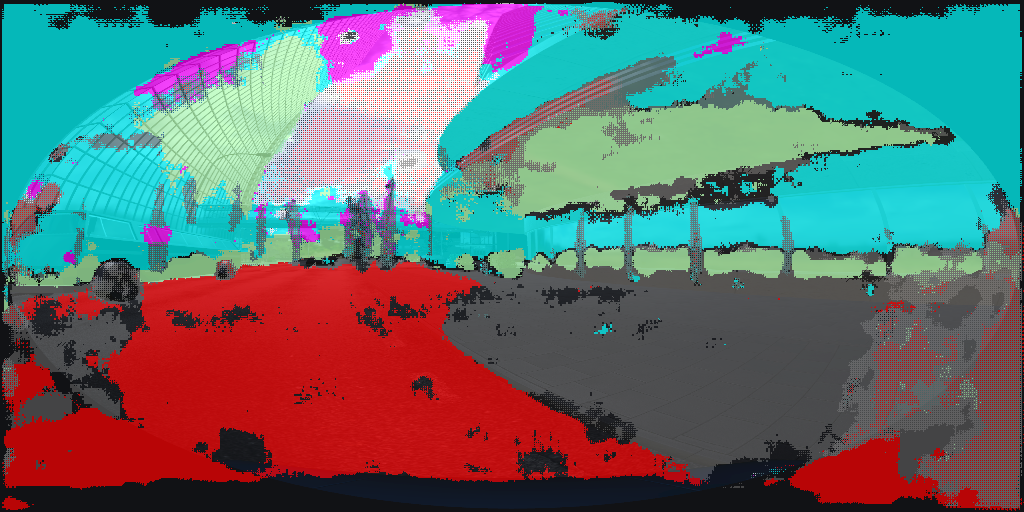
\includegraphics[width=0.3\textwidth]{949_pred2.png}}
    \subfigure[]{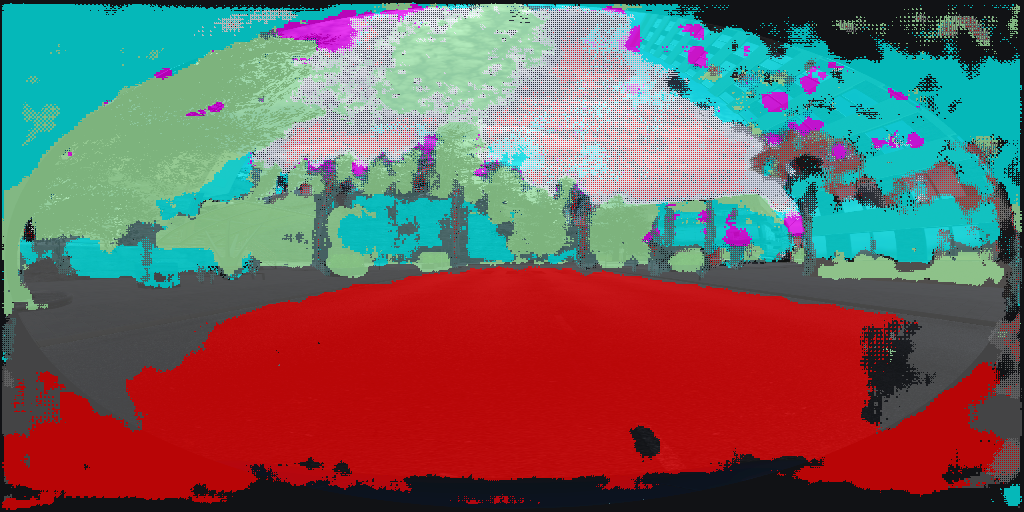
\includegraphics[width=0.3\textwidth]{1296_pred2.png}}
\caption{Predicted labels from Enet} \label{unityp2}
\end{figure}


\newpage

\section{Model evaluation on real dataset}


The main goal of this project is to detect free space in real images capture by fisheye lens. Hence, for the evaluation of the model, real world dataset called LMS Fisheye \cite{7471935} is used. The authors have used Fujinon FE185C057HA-1 fisheye lens which can capture FOV of 185 degrees.

For comparison, the E-Net \cite{Paszke2017ENetAD} model which was trained on pin-hole camera images of cityscapes dataset \cite{Cordts2016Cityscapes} was used to evaluate LMS fisheye \cite{7471935} images of road scenes. Some example ground truth images are shown in figure \ref{lmsgt}. The results of using E-Net model trained on cityscape images are in figure \ref{lmsp1} and the results of using our model trained on simulated images from Unity are as shown in \label{lmsp2}. The quantitative analysis is not performed due to unavailability of ground truth labels. However, looking at the results we can see that our model is performing better than the E-net model.

\newpage

\begin{figure}[h] 
    \subfigure[]{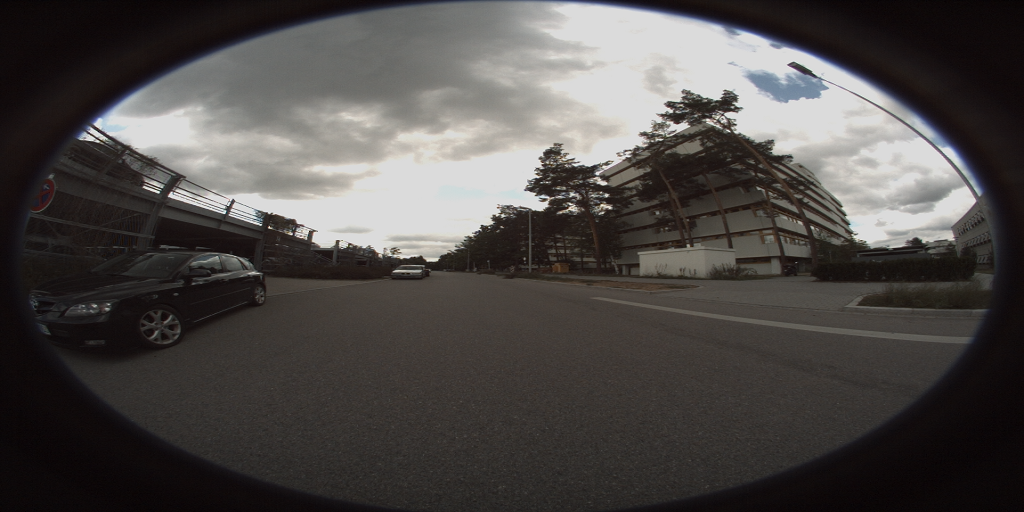
\includegraphics[width=0.3\textwidth]{DriveA_0001.png} }
    \subfigure[]{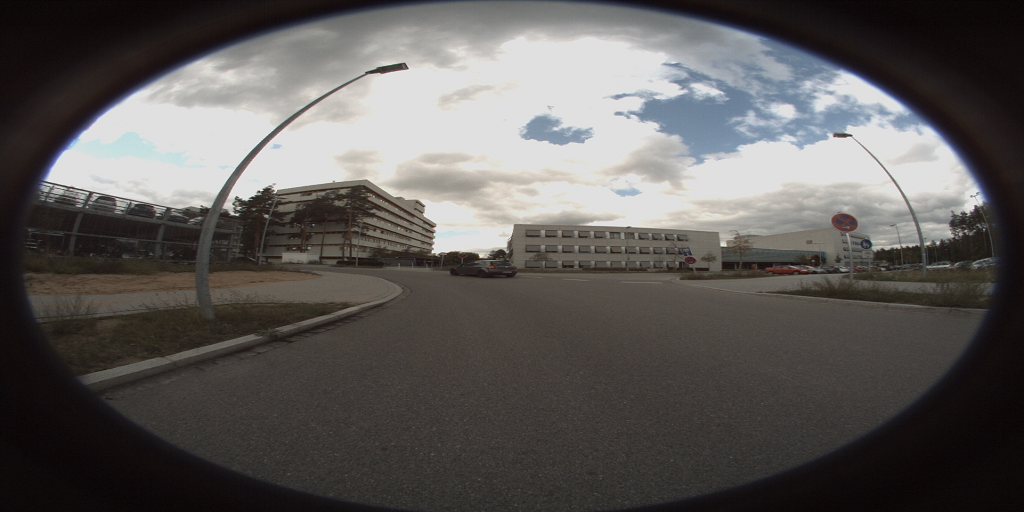
\includegraphics[width=0.3\textwidth]{DriveA_0084.png}}
    \subfigure[]{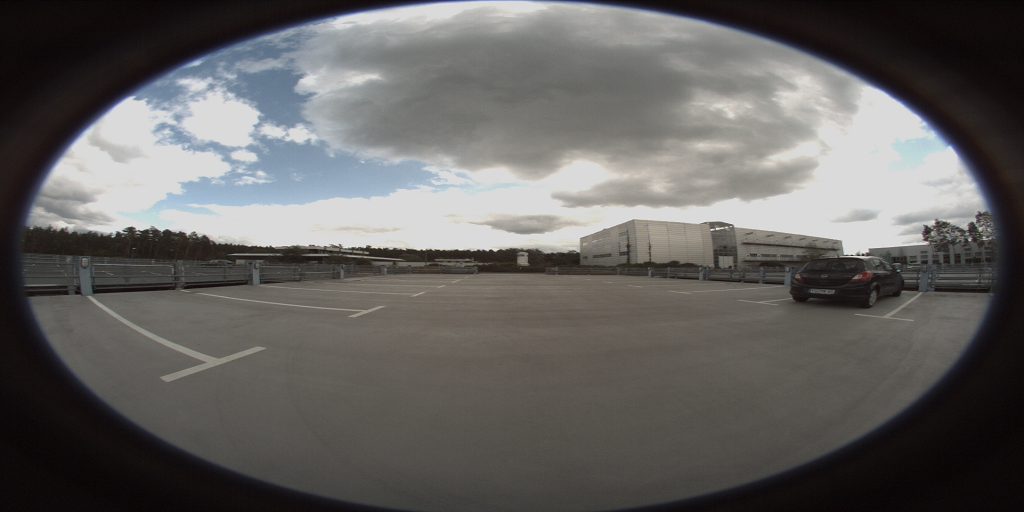
\includegraphics[width=0.3\textwidth]{DriveA_0883.png}}
\caption{LMS Fisheye groundtruth images} \label{lmsgt}
\end{figure}

\begin{figure}[h] 
    \subfigure[]{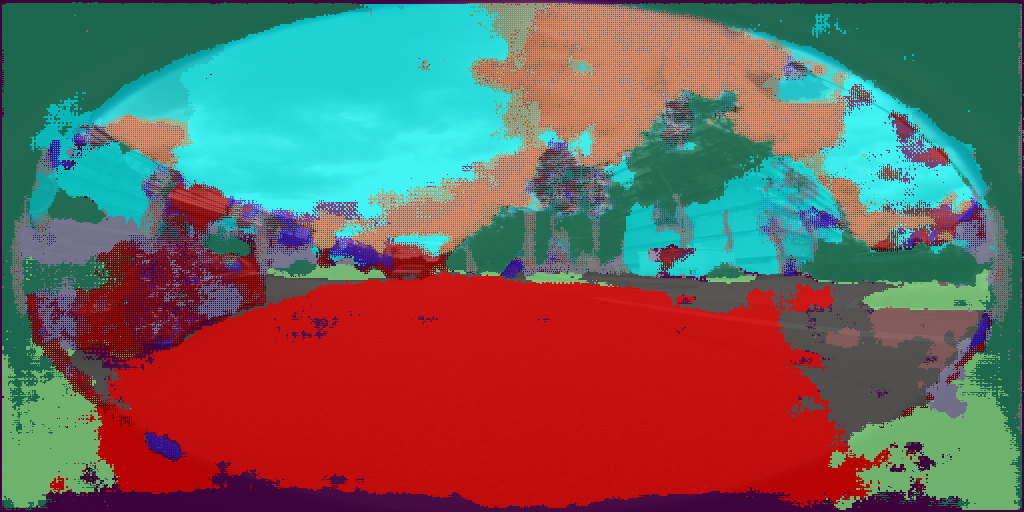
\includegraphics[width=0.3\textwidth]{DriveA_0001_pred.png} }
    \subfigure[]{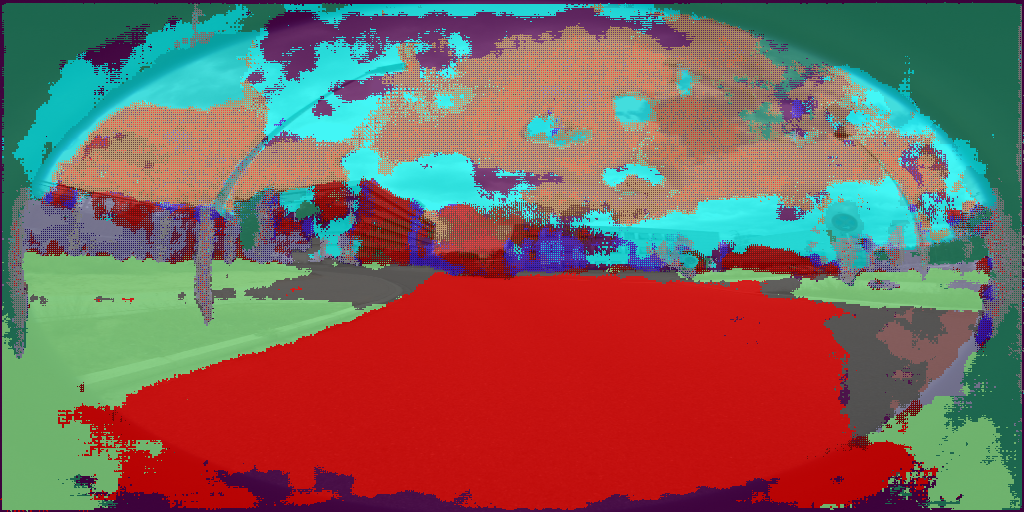
\includegraphics[width=0.3\textwidth]{DriveA_0084_pred.png}}
    \subfigure[]{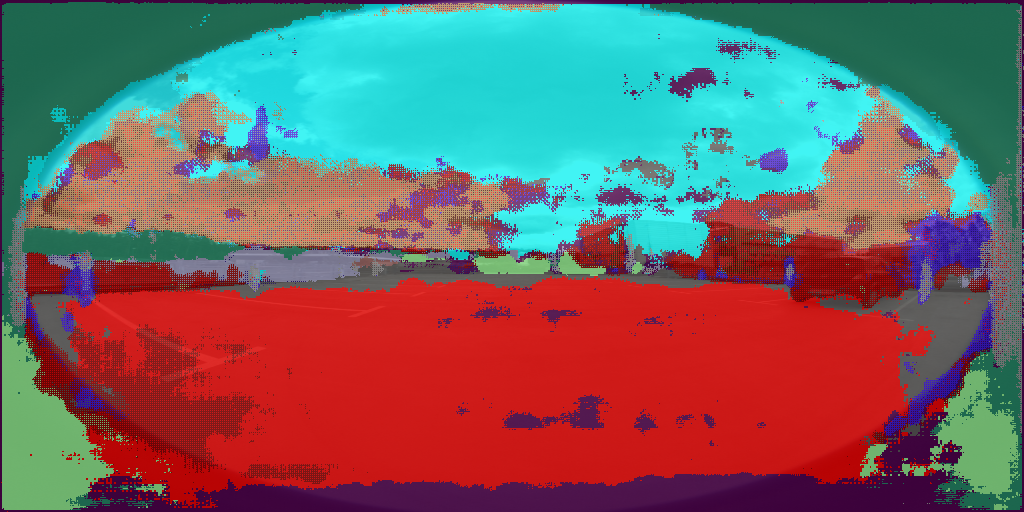
\includegraphics[width=0.3\textwidth]{DriveA_0883_pred.png}}
\caption{Results of using the E-net model trained on cityscapes} \label{lmsp1}
\end{figure}

\begin{figure}[h] 
    \subfigure[]{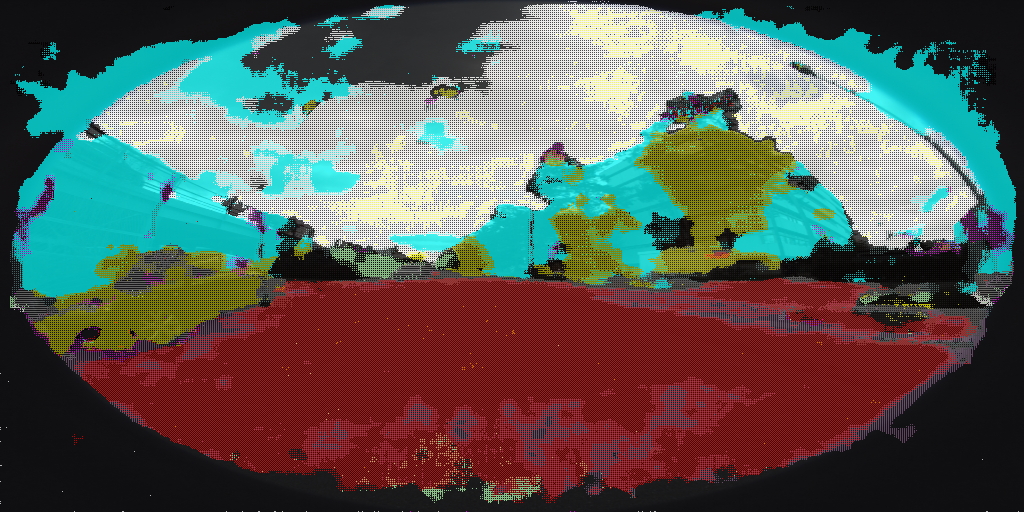
\includegraphics[width=0.3\textwidth]{DriveA_0001_pred2.png} }
    \subfigure[]{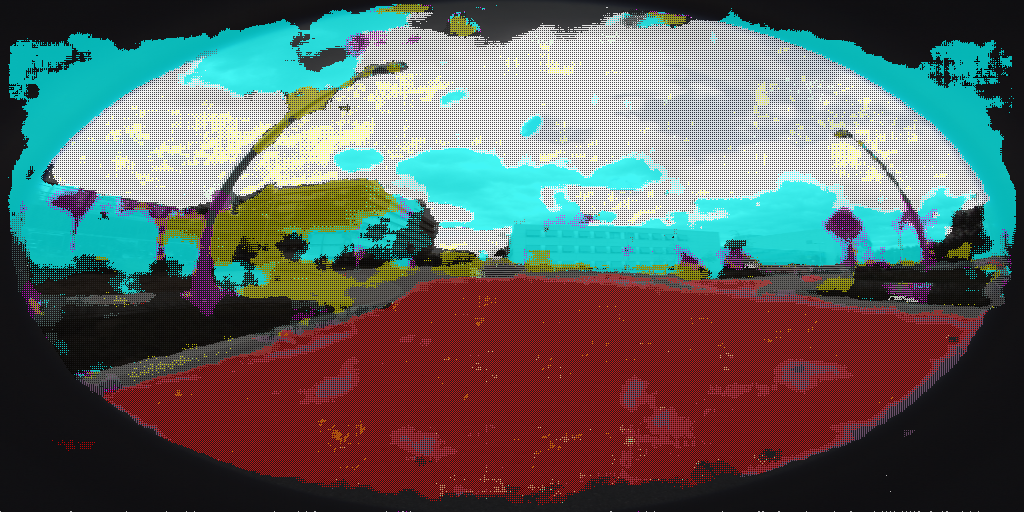
\includegraphics[width=0.3\textwidth]{DriveA_0084_pred2.png}}
    \subfigure[]{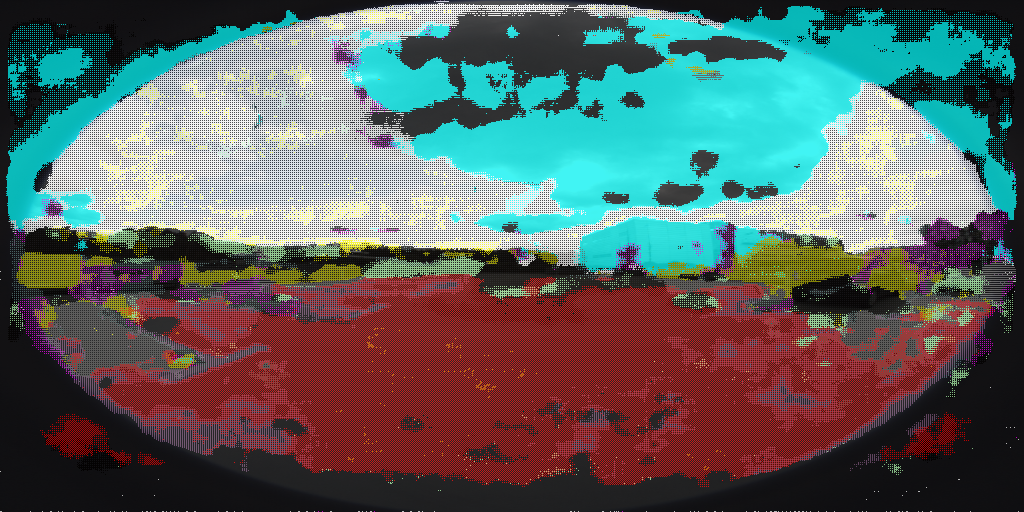
\includegraphics[width=0.3\textwidth]{DriveA_0883_pred2.png}}
\caption{Results of using our model trained on simulated fisheye images} \label{lmsp2}
\end{figure}




\chapter{Concluding Remarks}
%% Example of, how to use figures

\blindtext

\begin{figure}[h]
\centering

\includegraphics[width=0.6\textwidth]{TU_Chemnitz_positiv_gruen.pdf}
\caption{Graphic 1}
\label{fig:pic0}
\end{figure}

\blindtext
\blindtext

\begin{figure}[h]
    \subfigure[This is the first graphic]{
\includegraphics[width=0.49\textwidth]{TU_Chemnitz_positiv_gruen.pdf} \label{fig:pic1}}
    \subfigure[This is the secound graphic]{
\includegraphics[width=0.49\textwidth]{TU_Chemnitz_positiv_gruen.pdf}\label{fig:pic2}}
\caption{This is the caption of the whole graphic}
\end{figure}

\blindtext

 % Load Data from File example_figures

As seen in the results, our model clearly outperforms E-net on fisheye images. However, the model can be further improved by training on a larger dataset and by using better hyperparameters. Through this project, we demonstrated that simulation can be used to create images as well as labels when there is no labelled dataset available. Using this simulated dataset, we can train a neural network, either from scratch or through transfer learning to obtain good results. The trained neural network can then be used for inference in real world datasets thus solving the problem of unavailability of a labelled dataset. Also, through this project we demonstrated the importance of using fisheye cameras to better understand the surroundings in a autonomous car. We also showcased the potential of using Unity simulation to create any dataset for neural network training. Further work can be done on automating the dataset creation in Unity and also on using the neural network to drive the car inside Unity environment.

%---------------------------------------------------------
% bibliography based on Springer Design
%---------------------------------------------------------

\bibliographystyle{splncs03}
\bibliography{./src/enet}

\printindex

\end{document}
